\documentclass[12pt,french]{report}
%\usepackage[T1]{fontenc}
%\usepackage[utf8]{inputenc}
\usepackage{lipsum}
\usepackage{fontspec}
%\usepackage[french]{babel}
\usepackage{polyglossia}
\setdefaultlanguage{french}
\setotherlanguage{german}
\usepackage[french=guillemets]{csquotes}
\usepackage[
backend=biber,        % compilateur par défaut pour biblatex
bibencoding=utf8,
sorting=nyt,          % trier par nom, année, titre
%citestyle=authoryear-ibid, % style de citation auteur-année
citestyle=authortitle-ibid,
bibstyle=alphabetic,  % style de bibliographie alphabétique
autocite=footnote
]{biblatex}
\addbibresource{valbib.bib}


\usepackage{siunitx}
\setcounter{secnumdepth}{3}
\setcounter{tocdepth}{3}
\usepackage{textcomp}
\usepackage{graphicx}
\usepackage{pdfpages}
\usepackage{nomencl}
\usepackage{xcolor}
\usepackage[final]{pdfcomment} % nettre 'final' pour enlever les commentaires
\pdfcommentsetup{opacity=0.4}

\hypersetup{
	colorlinks,
	citecolor=black,
	filecolor=black,
	linkcolor=black,
	urlcolor=black,
	bookmarks=false
}
%\usepackage[colorlinks=true, %
%	linkcolor=cyan]{hyperref}
	
\usepackage{marginnote}

\makeatletter
%%%%%%%%%%%%%%%%%%%%%%%%%%%%%% LyX specific LaTeX commands.
\DeclareFontEncoding{LGR}{}{}
\DeclareRobustCommand{\greektext}{%
  \fontencoding{LGR}\selectfont\def\encodingdefault{LGR}}
\DeclareRobustCommand{\textgreek}[1]{\leavevmode{\greektext #1}}
\ProvideTextCommand{\~}{LGR}[1]{\char126#1}


\@ifundefined{date}{}{\date{}}
\makeatother


\title{Transformation de l'écoute\\ en musicothérapie}
\author{Valérie Gaillard}

\begin{document}
\maketitle
%%\title{{*}}

%\maketitle
\begin{titlepage}
 \begin{center}
    {\Large
     Zürcher Hochschule der Künste ZHdK\\
 	en collaboration avec l'Interkantonale Hochschule für
        Heilpädagogik HfH \\
	 Upgrade MAS in Klinische Musiktherapie \\ Master of Advanced Studies en musicothérapie clinique\\}
  \vfill
  {\Huge \emph{Le potentiel du test d'écoute Tomatis\textsuperscript \textregistered  pour la 
  musicothérapie} 
  	\vfill%Essai et réflexions en musicothérapie\\ sur des sujets souffrants de troubles de l'humeur 
  %au moyen d'un test d'écoute}
} \medskip


{\LARGE The Potentiel of the Tomatis\textsuperscript \textregistered Listening Test for  Music Therapy } 
\vfill

{\Large Mémoire pour l'obtention du titre de\\ \medskip
Master of Advanced Studies in Klinische Musiktherapie \\ \smallskip 
présenté par Valérie Gaillard}

{\large Directrice de mémoire : Bettina Kandé-Staehelin}



	 \hfill \\
	 \rule{0mm}{1pt} \hfill
{\large Zürich, novembre  2020}
 \end{center}
\end{titlepage}

% !TEX root = ./master.tex

\begin{abstract}
	\centerline{\textbf{Abstract}}
	\begin{french}	
\textbf{L'axe principal} porte sur la comparaison de la faculté d'écoute des patients avant et après 
la  musicothérapie.
\textbf{Les outils:} le test d'écoute Tomatis et le questionnaire WHOQOL sur la qualité de vie sont 
utilisés 
pour synthétiser les différences  pré/post traitement.
 %Des graphiques de courbes d'écoute synthétisent des différences pré/post traitement.
 13 patients, avec difficulté de régulation des émotions, sont répartis en 2 groupes: 6 patients avec la  
 musicothérapie et  7, de contrôle.
 % Le WHOQOL est rempli avant et 
 %après séjour afin d'évaluer leur état psychique.
\textbf{Résultats:} l'analyse comparative des résultats révèle une modification positive et significative 
d'écoute pré/post traitement %par le 
%test 
%d'écoute 
%Tomatis
 pour le groupe de 
musicothérapie, confirmée par le  WHOQOL, contrairement au groupe contrôle où la transformation est
faible et le questionnaire majoritairement négatif. % avec des valeurs plus 
%élevées. 
%Pour le groupe contrôle, la transformation a été faible et le questionnaire majoritairement 
%négatif.
\textbf{Conclusions:} la musicothérapie a eu un impact positif sur la transformation de l'écoute, corrélée 
à l'état psychique mis en évidence par le WHOQOL.
\textbf{Remarque:}  la totalité des tests d'écoute et des questionnaires demeure 
inférieur à ce qui avait été initialement planifié, et, en dépit d'une plus ample dimension statistique, ce 
travail avantagera plus les aspects qualitatifs que quantitatifs. %d'être 
%statistiquement significatifs, rendant notre travail plus qualitatif que quantitatif.
%Ayant tout à fait conscience des compétences scientifiques qu'une telle étude aurait exigé, ce travail 
%oscillera 

\textbf{Mots-clés: musicothérapie; écoute; son; oreille; test}
\end{french}

\begin{english}	
\textbf {The main axis} is about the observation by comparison of the auditory perception faculty of 
patients during the outcome of music therapy.
\textbf{Tools:} Tomatis listening test and WHOQOL quality of life questionnaire.
Listening curve graphs summarize the difference before and after treatment.
13 patients with the same type of pathology (difficulty in regulating
emotions) are divided into 2 different groups: one experimental group of 6 patients following music 
therapy, and one control group of 7 patients. Patients fill out the WHOQOL questionnaire before and after 
treatmenas to determine the impact or the lack of impact of the therapy on their listening.
\textbf{Results:} analysis of observation shows a positive and significant modification for the music 
therapy group regarding the WHOQOL test. The post-therapy questionnaire indeed shows an increase in 
values compared to the pre-therapy one.
For the control group, the transformation was weak and the questionnaire was mostly negative.
\textbf{Conclusions:} Music therapy had a positive impact on the transformation of listening, correlated 
to the psychic state, as the WHOQOL questionnaires results clearly showed.
\textbf{Note:} the small study added to the final number of WHOQOL lower than expected prevent our 
results from being statistically 
significative.
% the final number of listening tests and WHOQOL test was found lower than expected. 
%Added to the fact this was a small study. This therefore prevents our results from being statistically 
%significative. 
%Being fully aware of the scientific skills that such a study would’ve required, 
This work will oscillate more 
towards the qualitative aspect of the study than the quantitative.
\textbf{Keywords: music therapy; listen; sound; hear; test}
\end{english}
\end{abstract}













%\begin{Remerciements}

\tableofcontents
\listoffigures
\chapter{Introduction}

La musique vient dans la chair.

\begin{quotation}
 La musique vient dans la chair comme un produit immatériel
 qui vient travailler la zone a soigner. (...)      Je pompe de la
 guérison. (...)
Depuis le début des écoutes, j'ai la sensation physique et
 psychique de la
 transformation. (...)  La musique est équilibrante et guérisseuse, ma zone
 anesthésiée se remet à vivre, elle est remise en activité. (...)
 Il y a comme un consentement cellulaire. (...)
La béance s'estompe, cette
partie redevient comme les autres. (...)
Apaisement. Consentement. Réconciliation.    
% (...). [\dots]\, >>
$\ldots$\  Une patiente\autocite{propos d'une patiente}
\end{quotation}

Nous avons été très sensible au témoignage de cette patiente dont le
processus a été porté par le son et l'écoute. Le son l'a touchée intégralement et  a eu un impact sur sa transformation physique
et psychique.
Avec l'image évoquée du
consentement cellulaire, nous pourrions faire le
parallélisme entre l'entrée des sons dans la sphère d'écoute et la variation de la 
perméabilité cellulaire en cytologie. Si les sons réussissent à pénétrer dans la
cellule, il peut y avoir amélioration des échanges, un mieux-être et de la
communication.

Mais comment détecter la façon d'entendre du patient?
Comment comprendre les raisons pour lesquelles il y a imperméabilité aux
échanges, un refus des sons et une fermeture au monde si ce n'est en testant
son écoute?  Son écoute pourrait-elle nous donner certaines clés dans sa
compréhension? D'autre part, serait-ce  possible  par un test d'écoute
de marquer et souligner l'importance du processus musicothérapeutique? 
Il jouerait un
rôle de
révélateur de cette notion si abstraite et si primordiale qu'est l'écoute.
Ce sont les questions auxquelles nous avons tenté de
répondre dans ce travail.


Être au diapason, en harmonie avec soi et les autres
nécessite une écoute afin de nous accorder ou réaccorder à l'univers.
Car en définitive, nous sommes les
descendants de la cristallisation de la musique primordiale de
l'univers, selon
David Elbaz.  \footnote{David Elbaz, astrophysicien, chef de laboratoire au CEA et Alain
Destexhe, chercheur en neurosciences intégratives et computationnelles
à l'Institut  NeuroPsi de Paris Saclay} \autocite{delbaz_recherche_2016}

 



Si la musicothérapie a pour objectif d'apporter un soin aux patients, notre  approche se différencie par le fait de
vouloir mieux la mettre en valeur par des preuves
autres que celles rapportées par les patients. Fort nous a été de
constater un manque d'outils pour son évaluation. Car quelle que soit la technique utilisée, quel que soit
le traitement sonore, on espère une modification, on la suppose, la constate
 mais
 on ne la quantifie que difficilement. C'est la raison pour laquelle
 nous nous sommes servis d'un test d'écoute
 spécifique de la méthode d'Alfred Tomatis, choisi car puisant ses
 sources en audiologie. Faisant fi des critiques --
 ce ne sera pas l'objet de notre débat -- et  tout à fait conscients des
 grandes divergences d'opinion entre les adeptes d'une musicothérapie
 traditionnelle et cette méthode, (bien que le lien qui les unit est la musique), ce test particulier  nous servira à
 souligner l'importance de la musicothérapie 
 sur la transformation de l'écoute.
 Car ce n'est qu'après plusieurs
années de pratique et d'expérience que nous avons commencé à saisir
l'essentiel de la validité de ces théories.

Quoique nous n'ayons pas pu réunir toutes les données nécessaires
aux tests réalisés, - car nous ne sommes pas dupes qu'un vrai travail
nécessite beaucoup plus de précisions-, il nous a été possible toutefois d' étayer
les résultats obtenus, de recueillir quelques considérations hypothétiques par rapport à un
travail thérapeutique et de nous ouvrir à des réflexions. 
Grâce à Sandra Lutz Hochreutener,  \footnote{Dr. Sandra Lutz
  Hochreutener. Lehrt Musiktherapie und in der Weiterbildung – Tätig
  im Departement Musik. Funktion Co-Leitung und Dozentin Bereich
  Dossier, ZhDK}
 nous avons été encouragés à toutes les énoncer, pour pouvoir mettre un jour un terme à ce travail!


 

  


\section {L'hypothèse}


   La
   multiplicité des suppositions ayant trait au constat d'un manque
   d'outils d'évaluation objectif des résultats issus de la
   musicothérapie  nous a  permis de relever les questions
   suivantes:  



 
 \begin{itemize}
 \item  Question:
   Est-ce que l'écoute est visible et quantifiable par
          l'analyse d'un test?
 
 \end{itemize}
 	
 \begin{itemize}
 \item Question:
   Dans l'affirmative, y-a-t-il transformation?
   
\end{itemize}
 
\begin{itemize}
          
 \item Questions:
   Si cette modification existe, possède-t-elle un lien direct avec une prise en charge
  en musicothérapie?
  
  \item Dans l'affirmative, 
   si cette transformation est visible, est-elle en 
 	concordance 
 	avec celle de l'état psychique du patient?
        
 \end{itemize}

 






 

\section{Méthode d'étude}

	Nous utiliserons deux tests différents : 
	le test d'écoute spécifique d'Alfred Tomatis
	et le test-questionnaire, le WHOQO-Bref; tous les deux sont
        qualitatifs et quantitatifs.

        
        Ce test d'écoute détecte la manière de recevoir
        l'information. Nous obtenons une  
	représentation graphique générale des courbes de l'écoute
        (équilibre, déséquilibre, harmonie) obtenue à partir des seuils d'écoute
        calculés selon les fréquences et le volume que le sujet entend. Il s'en suivra une interprétation
        selon un procédé de lecture des zones de fréquences relevées.
	A cet effet, nous utiliserons l'appareil conçu à partir de 1950 par Alfred Tomatis, médecin
        O. R. L.: le Hearing Test,ou TLST, testant
        l'écoute.
	Nous procéderons en début et en fin de thérapie
        afin de recueillir les résultats des
        deux tests dans le but d'établir une comparaison.
        Nous spécifions qu'aucun support de la méthode conçue par
        Tomatis n'interviendra pendant les séances de musicothérapie.
        Cela n'impliquera ni 
\textsl{Oreille
	électronique} ni musiques préparées et filtrées. Leur
      fonctionnement et leur utilisation seront expliquées lors du
      chapitre sur la méthode, mais nous n'en ferons aucun
      usage. L'objectif est de mettre à profit cette façon de  tester pour constater
      s'il existe un changement dans l'écoute du sujet et de
      se limiter à ce support graphique, tel un ``dessin'',
      une image qui nous fournira des critères d'analyse.
       
	
	
        
   Le WHOQO--Bref ( World Health
   Organisation Quality of Life Assessement). Il s'agit d'un test d'évaluation de la qualité de vie, issu du
	programme de l'Organisation Mondiale de la Santé, l'OMS.
	Ce questionnaire est réalisé en parallèle supposée rempli par les patients eux-même  avant et après la thérapie.
	Il s'agit d'une vérification qualitative qui nous permet
        d'avoir l'opinion des patients sur leur processus de travail
        et  pour constater s'il y a une correspondance dans 
        les résultats obtenus avec le test d'écoute. 
	
	
	 
\{Plan du travail}

Nous aborderons en première partie l'aspect théorique : la musicothérapie, l'écoute, le son, l'oreille, le 
test d'écoute, les différents tests d'écoute en musicothérapie.  Ensuite, nous 
expliquerons  la méthode Tomatis
et puis, beaucoup plus en détails, son test d'écoute.
 
En deuxième partie,ce sera l'aspect clinique : les tests d'écoute réalisés  avec deux groupes 
de patients en parallèle, l'un de contrôle (GC) et l'autre d'intervention.(GI)

Et finalement suivront la vérification de l'hypothèse, les conclusions et 
interrogations. 


	


\
\chapter{La musicothérapie}


La musicothérapie est une pratique ancestrale qui existe depuis des
temps immémoriaux dans les mythologies et dans les rites. Dans l'Antiquité, que ce soit en Chine ou dans le monde arabe 
médiéval, nous relate François-Xavier Vrait,  	 
les vertus de la musique sont reconnues et considérées comme une évidence depuis 
fort longtemps. 
  \textquote{La théorie des nombres 
(``l'\underline{\underline{harmonie}} peut se calculer") est intégrée et infléchie dans la 
philosophie et les traités musicaux [\dots] et les formes d'utilisation 
thérapeutique de la musique sont décrites dans un ``traité de politique", 
``Kitab as Siyasa" [\dots] document syrien ou sabéen de la fin du 
\textsc{viii}\ieme\ siècle.}\autocite[ch. III, p. 
96]{vrait_musicotherapie_2018}.
La musique, la matière sonore, était  reconnue en quelque sorte comme étant d' utilité
publique, 
par les  politiciens  et les philosophes dans le but d'atteindre un
équilibre personnel et une harmonie civique.
 	 
A juste titre, l'Association Suisse de Musicothérapie suisse met particulièrement en relief 
la communication dans sa définition. Elle l'a décrit comme un 
 
\begin{itemize}
\item \textquote{processus thérapeutique, pour entrer en communication
    avec soi-même et pouvoir ensuite mieux percevoir le monde qui nous
    entoure, communiquer et s'exprimer.\autocite{site_musitherapy}}
\end{itemize}

La communication avec soi-même et avec l'autre est en effet un des
points 
d'une extrême importance dans l'équilibre psychique de l'homme, reflet
de 
l'harmonie entre l'intérieur et l'extérieur. L'harmonie est un des  
critères révélateurs qu'il nous sera donné de visualiser par le test
d'écoute (entr'autres, l'équilibre entre deux formes de perception) et sur
lesquels 
nous nous appuyerons  
dans ce travail.  \footnote{Le terme "harmonie" reviendra lors de
  l'analyse des tests Ch. 8 et 11}


 Au fil des siècles, de nombreux autres 
textes évoquent les liens de la musique avec la médecine, de sa place dans les 
rituels thérapeutiques et notamment en psychothérapie fin \textsc{xix}\ieme, 
début \textsc{xx}\ieme\ siècle. \footnote{Voir \ref{musicothEtpsycho},
  p. \pageref{musicothEtpsycho}.}.
Selon Aurelia Sickert-Delin, la musicothérapie 
psychologique doit être différenciée de celle dite médicinale qui 
\enquote{\emph{exerce une action 
énergétique, physiologique}} [\dots] avec \enquote{\emph{des effets curatifs}}  
ainsi que de celle dite \enquote{\emph{musicale, artistique}}. 
% \enquote{\emph{L'artiste-musicien éveille l'\,``artiste intérieur'' que l'être 
%en souffrance porte en lui, pour lui permettre de s'auto-guérir [\dots] par 
%l'écoute, l'expression et la création.}}\autocite[ch. 1,  p. 14, du texte 
%inédit communiqué par A. Sickert-Delin, musicothérapeute à Alersheim, rapporté à J. 
%Viret]{viret:b}

 De fonctionnelle, analytique, mo\-da\-le,  à 
struc\-tu\-rale, la musicothérapie se retrouve actuellement 
 à un tournant décisif où elle devient 
 \emph{intégrative} tout en conservant ses racines séculaires. Elle est 
intégrative dans le sens où elle permet un travail d'élaboration psychique dans une perspective de structuration identitaire \autocite[ch. III, p. 53, 
105]{vrait_musicotherapie_2018} et dans celui de l'intégration des données 
neuroscientifiques.
 
% Selon M. 
%Schneider \blockquote{elle cherche à sauvegarder et à fortifier la pure 
%substance sonore de l'homme\autocite[Voir tome I, pp. 202--203]%
%	[M. Schneider, <<Le rôle  de la musique dans la mythologie et les rites 
% des civilisations non européennes>>]{schaeffner.ea:histoire}.}


 
\paragraph{Musicothérapeute et neuroscientifique: }

 
Les musicothérapeutes sont souvent musiciens mais conjugent plus
rarement dans leur profession
médecine ou neurosciences. De leur côté, les neuroscientifiques appuient
et renforcent la crédibilité de l'action du son sur notre cerveau, via
l'oreille, en démontrant ses effets par un moyen technique
\textbf{visuel} que représente par exemple l'IRMfct. Mais, sans être musicien ou
musicothérapeute, leur découverte est plus rarement intégrée
directement dans leur pratique car hors contexte relationel d'une
séance, sans l'aspect intuitif et impalpable de cette forme de prise
en charge.
Il est malheureusement ardu d'être très compétent dans ces deux domaines
de pointe de façon simultanée.   \footnote  {Il existe toutefois certains chercheurs
comme Emmanuel Bigand ou Hervé Platel qui font exceptions.}

Car l'aspect fugace du son, de la musique, de ce médium volatil et
intemporel par
définition, n'amène pas à tout un chacun le
même aspect concret que peuvent témoigner des supports
graphiques. Ceux-ci sont des 
reflets d'un espace-temps du travail d'élaboration
psychique d'un patient, sur lesquels l'art-thérapie, par exemple, s'appuie et trouve
ses sources.


Néanmoins, il y a l'enregistrement sonore des séances qui 
permet d'avoir un support concret et solide, comme le pratiquent Edith Lecourt, ou Carole et Clive 
Robbins. \footnote{``Les Art-thérapies'', pp88--117, Ed.Armand Colin}
Les séances sont écoutées, filmées pour une
analyse la plus objective possible; on donne 
une forme et un sens aux sons recueillis pour les retracer dans le
parcours du patient (avec ou sans sa présence). Par contre, cette analyse  restera
tout de même très subjective de par sa nature (le son ne laisse pas
de trace) et de par la nécessité de la présence d'autres formes d'
écoutes (celles du thérapeute).

Peut-être pouvons-nous nous imaginer que l'avenir apportera d'autres outils
directement accessibles pendant les séances, afin
 de, si nécessaire, visualiser directement l'effet en temps réel de la musique sur le
 cerveau:  imager couramment et facilement la manière d'ouïr de chaque
 patient peut se révéler important, complémentaire et intéressant pour l'anamnèse et la prise en charge.
 Ce serait l'image de la
 physiologie de l'audition personnalisée à chaque séance.

 
Vivant dans un monde très visuel, les preuves sous cette forme sont
validées pour soutenir l'argumentation du bien-fondé d'une thérapie.\footnote{
	\pdfcomment{Faire une phrase}les critères de l'EBM (evidence based medecine, médecine basée sur des 
        preuves) F. X. Vrait, ch. II, pp. 105--106 }
On veut voir pour croire. Est-ce 
notre esprit formaté cartésien depuis quelques centaines d'années qui nous 
empêche de penser différemment? 
Actuellement, c'est une nécessité due à notre époque pour crédibiliser l'impact 
du son sur notre être.


Si la 
musicothérapie a un impact certain sur la façon d'écouter en
entraînant sa 
modification, elle peut être  
démontrée et démontrable, \textsl{objectivée},
sous la forme simple d'un test, comme saisie par 
l'\oe il neutre de l'objectif d'un appareil
photographique.

Cette hypothèse formulée va être donc l'objet de notre étude qui
débutera par la notion d'écoute que nous allons revisiter.
 

\chapter{Aspects neurophysiologiques du son et de l'écoute}


\section{Le son}

Lors d'un concert, si nous pouvions visualiser les sons qui
s'échappent de l'orchestre, ce serait un chatoiement de cercles qui se
répandraient tout autour de nous, comme 
la propagation des
ronds dans l'eau suite à un ébranlement de sa surface.
Les molécules d'air en contact avec la source sonore se déplacent et
créent une vibration. \autocite[p. 183]{bencivelli:pourquoi,}.


Le son peut être déterminé par différents paramètres
physiologiques et psychologiques.
Il est défini très précisément par un ensemble d'unités physiques chiffrées
: les décibels  et les hertz.\footnote{Voir Annexe: Le son et sa
  définition.}




\section{Ecoute, perception des sons et troubles associés}
\paragraph{Ecouter ou entendre : une différence}

La définition du verbe `entendre' et du verbe `écouter' 
\autocite[pp. 361--385]{hachette:dictionnaire} nous paraît opportune
en raison de la confusion courante des deux termes :
\begin{description}
\item[Entendre] c'est  percevoir des sons, saisir par l'ouïe.
\item[Ecouter] a trois sens: 
\begin{enumerate}
	\item prêter l'oreille à; s'appliquer à entendre;
	\item prêter attention à l'avis de quelqu'un, suivre un avis;
	\item \emph{fig} suivre une impulsion,	une inspiration.
\end{enumerate}
\end{description}


Par les sources étymologiques du
terme `écouter' ,
 sa racine sanskrite \emph{ ``avih'' } se traduit par
 \emph{``évidence'' , ``connaissance'', ``discernement''}. Puis, en ancien
 français, ce mot a donné \textit{``oüir''} signifiant aussi bien \textit{``entendre''} ,
\textbf{`` écouter'' } que \textit{``comprendre''}.\footnote{Source:``Etymologie Français latin grec Sanskrit-Google Sites'' }.
 Est-ce la raison
pour laquelle il subsiste toujours un amalgame 
sur le sens de ce verbe?
Selon Didier
Colin \footnote{Didier Colin,2015 ``Interprétez vos rêves''}, cette faculté
permet non seulement d'écouter et de comprendre avec plus d'attention
mais aussi de percevoir des sons et peut même, être doué de
\textit{``clairaudience'}'. 


En définitive, \emph{entendre} est une attitude passive par rapport au monde sonore
qui nous entoure. Nous recevons les sons sans les interpréter et cela
ne demande aucun effort. C'est une action involontaire et non
sélective.

\textit{Entendre} nous spécifie Bernard Auriol, \autocite[p. 2, ch . 1]{auriol:cle}
\begin{quote}
	<<\,suppose un son (physique), une oreille
	pour le capter, un système nerveux pour le recevoir.\,>>
\end{quote} 
Tandis qu'\textit{écouter} 
\begin{quote}
	<<\,est un
	processus actif supposant préférences et répulsions pour tel son ou
	telle séquence sonore.\,>>
\end{quote}


Entendre et écouter sont donc  «\,deux
fonctions essentiellement distinctes bien qu'évoluant apparemment sur
des terrains identiques\,>>
% ancien texte {\textbf{site internet: http: auriol.free.fr} Extrait de l'entretien réalisé par
%	Bernard Auriol avec Alfred Tomatis, 1973.}.
[\dots] avec «\,l'élément conscient, facteur essentiel sur lequel repose toute la
différence entre ces deux activités\,».\autocite[]{tomatis_oreille_1991}
\pdfmargincomment{Pages des 2 citations?}
\begin{quote}
	
	<<[\ldots] \emph{Entendre, c'est en quelque sorte subir
		un son} ou un message qui nous est adressé. \emph{Ecouter, c'est désirer appréhender ce son} ou ce message [\ldots]>>
	\autocite{tomatis:education}.	
\end{quote}

Selon J. Auriol \autocite[18] {auriol:cle} et Tomatis(\autocite[52]
{tomatis:loreille}, l'écoute est un `` éveil auditif''  défini avec au
minimum trois
fréquences simultanées ( dans le sens esthétique). Il s'agit donc d'un phénomène
complexe avec la corrélation d'axes
linéaires (notion temporelle) et verticales (notion spatiale), doublée d'une
dimension psychologique.

En effet, si \enquote{\emph{Je suis la musique que je fais ou écoute}}\autocite{viret:b}, \textbf{écouter} implique 
une conscience pour s'actualiser dans le sujet. \footnote{Voir point
  \ref{jeSuisLaMusique:viret}, p.2 \pageref{jeSuisLaMusique:viret}.}
Elle est une opération 
qui suppose une participation active dans le choix du message
ou dans la sélection d'une voix. Elle  implique la volonté,
\pdfmargincomment[color=green]{Bien!}
permet une forme de décodage: il s'agit d'une capacité.
Dans un milieu sonore important,
 bruyant, comme un café, lorsque nous lisons attentivement, nous faisons abstraction
des bruits environnants; en soi, nous les entendons parfaitement mais nous n'y
prêtons pas attention. Nous parvenons à couper les sons parasites, à nous en abstraire pour
nous concentrer uniquement sur les plus  pertinents, en l'occurrence
ici ceux de notre lecture intérieure.




  En creusant encore la racine du mot `écouter', celle-ci signifirait aussi \emph{partager}; nous
  remarquerons alors à juste titre que nous écoutons le plus souvent en
  face de quelqu'un dans le but de dialoguer, d'échanger. Le même
  phénomène se réalise avec un livre qui transmet et partage des
  connaissances. L'écoute permet donc la communication, sous-entend le
  plus souvent la présence d'un être en vis-à-vis et nécessite de la
  concentration. Il faut cette volonté inclue dans celle-ci  pour
  comprendre et rentrer en contact avec la voix de  l'écrivain qui
  chante dans le texte avec celle, intérieure, du lecteur.

  
 \textbf{Ecouter} se base certes sur une stimulation prenant sa source à 
l'extérieur mais devant être \textbf{ intérieurement et intentionnellement
	recherchée}.




      \paragraph{Ecoute musicothérapeutique}
      

Par extrapolation, nous pouvons aussi différencier les différents types d'écoute. D'après Edith Lecourt \autocite[ch. 10 <<\,De l'écoute verbale à l'écoute musicale\,>>, p. 182.]{lecourt:decouvrir}
 on en distingue plusieurs : l'écoute verbale, musicale, plurivocale et multiple.
 L'analyse musicale qui permet la différenciation d'une voix d'un ensemble polyphonique est appelée \emph{plurivocale}. Celle qui est multiple n'est pas analytique  mais 
 \begin{quote}
 	 [\ldots] \textit{ouvre une disponibilité, met en suspens les grilles verbale et musicale} [\ldots] \emph{pour parcourir le vécu sonoro-affectif}\autocite[p. 183]{lecourt:decouvrir}.
 \end{quote}
 Employée en musicothérapie, Edith Lecourt la nomme la technique de la  \emph{communication sonore} qui peut apporter 
 <<\,des ouvertures sur l'analyse des niveaux plus archaïques de l'organisation mentale\,>>\autocite[p. 154]{lecourt:decouvrir}.	
 Par l'expérience musicale en groupe, il peut y avoir un moment
 particulier, de ``grâce"  nommé ``le concept d'illusion groupale",
 l'illusion d'une unité absolue, comme un seul corps \autocite{anzieu:groupal} dont parle Didier Anzieu.


 
\emph{Ecouter} implique les notions de \emph{son} et
d'\emph{oreille}. Nous allons dans un premier temps approfondir  la
définition du son dont les caractéristiques physiques seront mis en
annexes et il en sera de même pour l'oreille et les détails
d'anatomie.\footnote{Annexes: Son et Oreille}

\







\paragraph{Ecoute objective ou subjective?}

Nous avons tous,
selon les manuels d'anatomie, la même
oreille, du moins nous pouvons reconnaître une analogie de structure. Nous devrions donc entendre et écouter la même chose
lors d'une même information diffusée tout comme le fait un enregistreur avec un micro. Pourtant il n'y a pas d'écoute \emph{passive}. Chacun n'entend pas de la même manière les mêmes
informations, chacun trie et fait son propre choix selon la fonction
d'écoute élaborée depuis l'enfance. Cette fonction sélectionne très
rapidement les mots pour être intelligible, pour se faire
comprendre. Nous rejoignons l'idée de Tomatis lorsqu'il affirme que
\textit{"L'oreille a un psychisme"} , car tout un chacun entend ce qu'il veut bien
entendre. \autocite{tomatis_oreille_1998} 
Nous transformons notre écoute selon nos attentes.

Allant dans le même sens, cet 
article d'une 
étude franco-américaine scientifique
\autocite{fritz_stradivarius} au sujet des célèbres violons
Stradivarius: faite avec un protocole 
d'écoutes en aveugle avec
des violonistes professionnels et en parallèle avec un public (caché
derrière un rideau), elle démontre que le mythe de la suprématie
de ces instruments extrêmement chers tombe au profit d'instruments
neufs.

Le cerveau 
transforme les informations reçues selon nos attentes et joue un
rôle majeur dans notre perception.
\autocite{lemonde.fr:stradivarius}.
% 
%\footnote{\href{http://www.lemonde.fr/culture/article/2014/04/10/le-stradivarius-detrone-par-les-violons-modernes\_4398681\_3246.html}{LeMonde.fr}.}.
\autocite[p. 43]{roque:lecoute}


 
En est-il de même lorsqu'il s'agit de patients souffrant de dépression
ou de burnout? Sont-ce justement les souffrances dues à des situations
insupportables qui
ordonnent à notre cerveau de se protéger en obscurcissant la
perception sonore?  Ne plus écouter certains
sons permettrait-il en quelque sorte d'échapper à la souffrance et de faire une
pause dans la douleur? Nous avons le droit et c'est un réflexe de
survie que de ne plus vouloir voir une scène affreuse et de détourner
notre regard. Nous pouvons supposer qu'il en est de même pour l'oreille ne voulant plus capter
certains sons.

Freud mettait déjà en évidence le phénomène de la
\textbf{sélectivité }comme ``mécanisme de défense''. \footnote{S.Freud,
  Psychologie de la vie quotidienne, 1904}

\textbf{\emph{Vouloir voir, c'est viser, vouloir entendre, c'est
    écouter.}}

L'\oe il regarde par la rétine et  vise, sous l'ordre du
cerveau, avec la macula. Dans la même idée, par l'écoute, nous avons
l'oreille et la cochlée (partie interne de l'oreille) qui permet
l'analyse des sons. Vouloir entendre dans le but d'écouter est comparable  à
la visée de l'\oe il lorsque l'on veut collecter une
information.
 


 \textbf{ L'audition est la capacité perceptive du système auditif et l'écoute, c'est ce qu'on en fait.}


\section{La perception des sons et l'existence de troubles
  émotionnels}


Conformément à l'idée que l'oreille nécessite d'être sollicitée pour
énergiser le corps et le cerveau en vue d'un épanouissement, la
capture d'un très haut nombre de stimulations par seconde (3G) agit
sur la formation réticulée,\footnote{Déf.: la formation 
réticulée est la partie centrale de la substance grise du tronc cérébral, 
constituée de nombreuses cellules nerveuses qui communiquent entre elles par de 
multiples jonctions appelées synapses.}
comme prouvé par d'incessantes recherches scientifiques actuelles,
confirmant la très grande complexité de notre cerveau.






                

\paragraph{ La dépression et l'audition dans le rapport
  musique-cerveau}

Depuis la plus haute Antiquité,  la reconnaissance de
l'impact de la musique sur l'émotion est actuellement confirmée par
des approches récentes, dont A.Damasio\footnote {{L'erreur de
    Descartes}, Antonio Damasio, Paris, 
Ed.Odile Jacob, 1997}, qui souligne l'indispensabilité de l'\textbf{émotion}
sur l'intelligence --  \textbf{intelligence émotionnelle et intelligence
cognitive --.}
En outre, les approches neuro-psychologiques sur les \textit{agnosies
  auditives}\footnote {Peretz
  I. \textit{in} Seron, Baron et Jeannerod \autocite[<<\,Les agnosies auditives\,>>,
  pp. 205--216]{seron.baron.ea:neuropsychologie}},
sur la perception distincte des émotions de la musique\footnote
{Platel H. 2002\autocite[pp. 223--224]{platel_neuropsychology_2002}}, 
sur l'apport de Bigand E.\footnote {Bigand E., chercheur, professeur 
de psychologie cognitive à l'Université 2013 \autocite[Ch. 3
p. 35, "Vous avez l'oreille musicale"]{bigand:cerveau} } soutenant le
manque de fonction biologique précise de la musique,
et sur la
découverte du rôle mimétique des\textit{ neurones miroir }( ``troisième''
cerveau) de Rizzolati G. (1990)\footnote{"Notre cerveau n'a pas fini de nous étonner", Entretien avec Jean-Michel 
     Oughourlian, pp. 118--119, Ed. Albin Michel, Le Livre de Poche
     2012} nous permettent de maintenir et
appuyer 
la fonction thérapeutique de la musique.








   

 
Quant au lien entre audition et dépression, d'autres perspectives
récentes mettent en lumière les évaluations de ces dernières comme les approches de Yowell (1995),\footnote{Yovell
  Y., Sackeim, H.A., Epstein, D.G., Prudlic, J., Devanand, D.P.,
  McElhiney, M.C., Settembrino, J.M. Bruder, G.E., 1995. Hearing loss
  asymmetry in major depression. J. Neuropsychitr. Clin. Neurosci. 7, 82--89.}Millot and Brand (2001) et 
Canbeyli (2010)\footnote{Canbeyli R., 2010. Sensorimotor modulation of mood and
depression: a integrative review.Behav.Brain.Res. 207 (2), 249--264} tous soulignant l'important\textbf{ lien entre la difficulté}
à \textbf{percevoir certains sons et la présence de troubles émotionnels,}
laissant entendre une correspondance sous forme de `` vase communiquant''
entre la \textbf{perte de reconnaissance de
sons et un état dépressif.}

Une autre étude du CNRS, (2009)\footnote{``Les seuils auditifs des sons purs 
	sont diminués chez les personnes déprimées avec des
	troubles de stress post-traumatique.'', <<\,Pure-tone auditory 
	thresholds are decreased in depressed people with post-traumatic stress 
disorder\,>>, Journal of Affective disorders. Recherche du CNRS en collaboration
	avec Tomatis Developpement S.A. Auteurs : Stéphanie 
	Aubert-Khalfa; Emmanuelle Reynaud; Myriam El Khoury;
	Olivier Blin - INCM, UMR CNRS 6193, Jean-Pierre Granier -
	TOMATIS DEVELOPPEMENT S.A. Eva-Maria Grosse; Jean-Claude 
	Samuelian - Pôle Psychiatrie Centre, La Conception Hospital.}mentionne l'effet des événements
traumatisants sur l'audition, impliquant des conséquences dépressives:
la double approche groupale (Gr en bonne santé et Gr déprimé avec
troubles de stress post-traumatique) met en lumière la diminution des
seuils auditifs (cf. test clinique, ch.6 p. 44) où on relève une augmentation de l'activité de la
première et deuxième aire auditive ainsi qu'une diminution significative des
seuils auditifs par voie osseuse (entre
\SIrange{275}{8000}{\Hz}) et en conduction aérienne
(\SIrange{500}{875}{\Hz} et  \SIrange{2000}{8000}{\Hz}).

\paragraph{Rapport entre audition et émission vocale}

En guise de complètement, le rapport entre audition et émission vocale
est enrichi par l'apport de Granier J.P. \footnote{psychologue, formateur
Tomatis, (Paris), co-auteur de l'étude CNRS des seuls auditifs et
dépressifs}
qui soutient qu'``Il existe une 
interaction
constante entre le traitement auditif \textbf{et} moteur de la
voix, entre l'information sensorielle \textbf{et} les programmes moteurs impliqués
dans la parole ou le chant.''
Le programme moteur qui a été déclenché
pour la parole permet au cerveau d'effectuer des tentatives d'anticipation
des émissions acoustiques imminentes, comparées à l'information
auditive reçue; cette boucle
auditivo-vocale/ verbale permettra, dans un processus circulaire, un ajustement.


Le nombre limité d'études musicothérapeutiques au sujet du \textbf{burnout}
nous invite aux travaux de Sigrist F., parlant de
\textit{``Resonanzstörung''} qui relève la connection neuronale directe et significative entre les systèmes auditif et
         limbique, d'où découle une activation émotionnelle et une
         résonance définie comme ``interpersonnelle''\footnote{"\textit{interpersonnelle Resonanz}"F.Siegrist F. Sigrist, médecin
psychiatre, psychologue et musicothérapeute à la Privatklinik
d'Hohewegg, Zürich.\autocite[pp.55--90] {sigrist_burnout_2016}.}.



Sans nous éloigner trop de notre sujet, nous pouvons rappeler
les difficultés observées sur les
\textbf{autistes} et leur capacité d'écoute cérébrale excessive et
incontrôlable investiguées par Harrisson B. et St-Charles, 2017\footnote{\autocite[Cet ouvrage propose une description unique du TSA
   (trouble du spectre de l'autisme
   pp. 22--23)]{harrisson.st-charles:lautisme} }. Dans ce tableau
 figure un trouble d'intégration sensorielle (TSA), où
 l'hypersensibilité aux sons devient douloureuse quand le flux excessif
 des
 informations empêche le tri,  protégeant ainsi le cerveau d'une surcharge.


Nous constatons ce lien puissant et indissociable  entre l'ouïe donnée
par l'oreille pour entendre et écouter et le cerveau exécutant ce
travail entre la 
parole et l'oreille.








\chapter{Différentes approches musicothérapeutiques: épreuves
  et tests}
Avant d'aborder le test d'écoute qui va nous intéresser plus
particulièrement pour notre travail, nous allons faire la différence
entre la définition du test et celle de l'épreuve.
Le test est normé, c'est une épreuve codifiée, numérisée, échelonnée,
statistifiée, comme celui du test d'intelligence de Piaget où il y a une
norme et des chiffres. Tandis que l'épreuve est plus globale, plus complexe,
demande plus de matériel et permet de
cataloguer mais n'est pas statistifiée.

Selon Doron et Parot, c'est en 1890 que le test (du latin ``testum''
signifiant ``pot de terre'') a été utilisé pour la
première fois. C'est un procédé d'évaluation qualitative ou
typologique des caractéristiques d'une substance, d'un corps et d'une
fonction.
Le test psychologique est une épreuve définie impliquant une tâche à
remplir, identique pour tous les sujets examinés, avec une technique
précise pour l'appréciation du succès ou de l'échec.
L'épreuve (action d'éprouver) est ce qui permet de juger la valeur
d'une idée, d'une qualité intellectuelle ou morale d'une personne.

La psychologie clinique s’intéresse moins
aux tests et plus aux à-côtés des tests, c. à d. aux réactions de la
personnalité à la situation à la fois matérielle et sociale dans
laquelle le sujet se trouve placé. L’épreuve spéciale analytique, quantitative, ne prend tout son sens que rapprochée d’autres épreuves analogues (comme dans le profil psychologique) intégrée dans le portrait psychologique global.Cette réciprocité de l’ensemble et du détail est une condition générale de la psychologie humaine : sur l’intuition d’ensemble initiale quelques faits particuliers viennent se profiler, l’image de l’ensemble est révisé et permet d’interpréter de nouveaux détails ; d’autres détails modifient à nouveau l’ensemble, et ainsi de suite.
L’analogie est frappante avec la médecine clinique : là aussi on a
espéré substituer à l’art clinique incertain une somme d’examens de
laboratoire ; mais là aussi il a fallu revenir à l’idée d’une
intégration des examens de laboratoire dans l’ensemble clinique.



\subsection{Définition du test d'écoute et de l'audiogramme}

De manière générale, le test d'écoute se trouve sous la forme verbale,
à caractère  
psychologique mettant principalement l'accent sur la communication
et la capacité d'empathie.

Dans le milieu médical, on le nomme test d'audition ou audiogramme. Il
sert à mesurer les seuils d'audition des sujets, grâce à l'audiomètre. Cet 
appareil français avait été mis au point en 1933. Les Américains
ont repris ces travaux pendant la dernière guerre pour pouvoir dépister
les dommages subis par ceux qui conduisaient des avions ou d'autres
engins similaires bruyants.
  L'audiogramme est une épreuve d'ordre physiologique. Ce test peut faire partie des examens  pratiqués en otologie\footnote{otologie : branche de la médecine
  	qui étudie l'oreille et ses maladies.} pour poser un diagnostic. 
   C'est un examen à partir duquel se
  dessinent les données dénommées étiologiques\footnote{étiologie : étude des causes
  	d'une maladie} pour détecter un trouble de la fonction auditive. Un pronostic pourra définir le mode de thérapie
médicale, chirurgicale, prothétique ou rééducative. La procédure
technique inclut des paramètres et manipulations propres au corps
médical des auscultations O. R. L. et  n'est pas systématique.






\section{Le test d'écoute en musicothérapie}

Les musicothérapeutes ne se lassent pas d'explorer l'alliage du son
 et de la psychologie, et vice
 et versa, les psychanalystes, les psychiatres, les psychologues
 s'intéressent à intégrer le son dans leur travail. Par ce truchement,
 une élaboration est faite, porteuse d'informations différentes que
 celles d'un questionnaire médical. Le son permet de donner un miroir
 psychologique de la personne par un chemin détourné. Avec cette dimension
 musicale, le test d'écoute diffère de certains tests psychologiques usuels
 et fait partie de ce que l'on nomme le \textbf{ bilan
   psycho-musical}. Celui-ci se déroule soit avec l'audition d'\oe uvres
 musicales où les patients répondent à une grille précise de questions
  soit en trois parties, avec un entretien,
 une écoute musicale (partie réceptive) et une production musicale
 (partie active).
Ce bilan permet d'évaluer la disponibilité du sujet pour cette
approche et permet au thérapeute d'évaluer l'intérêt dans ce cas
d'une telle prise en charge.
 On reconnait de plus en plus le rôle éminemment important que joue la musique
 dans les traitements psychiatriques et ce type de test devient
 fréquent dans beaucoup d' établissements. Ils le sont aussi par principe de précaution et
 par souci d'ajuster au plus près une
 musicothérapie.



  
\section{Les musicothérapeutes et leurs différents types de test}
\label{musicothEtpsycho}

	 La musique s'est révélée ainsi être un important support
         d'expérimentation et 
	 R.Benenzon,  Verdeau-Paillès, Edith
         Lecourt et H.Bonny ont su intégrer dans leur pratique l'utilisation du son comme
         élément facilitant l'exploration psychique.
         Ils ont su, chacun à leur manière  élaborer des procédures destinées à faciliter
         l'introspection et la communication.
\footnote{Nous pouvons aussi citer les recherches telles faites avec la reconnaissance de
bruits, de sonorités (G. Boissière), telle autre avec un test rythmique
(C.Holthaus) ou par celui
des réactions aux intervalles musicaux (Savioz PPIT).} 
Dans d'autres approches, comme F.Nevjinsky, B.Auriol, J. Bonhomme
           et A.Tomatis ont ainsi développé leurs propres
           concepts construisant plusieurs types de \emph{bilans musicaux},
           dont voici une brève énumération.
           

          

         

  \subsection{Benenzon Rolando Omar} 
	\textbf{ Buenos Aires, psychiatre et
    musicien argentin, (1939)}
	  \label{benenzon}
	  Dès 1969 il base sa technique 
	  musicothérapeutique sur des concepts 
	  de Jung, mais s'imprégnant de même de Freud, Winnicott (
          1953, concept d'objet transitionnel) \footnote{
          D. W. Winnicott: ``Jeu et réalité'', Gallimard 1975 }
          Watzlawick. \footnote{ Watzlawick Paul, 1921-2007  théoricien dans la théorie de la communication et le constructivisme radical, membre fondateur de l'École de Palo Alto, psychologue, psychothérapeute, psychanalyste jungien et sociologue} 
	  Influencé par les grands  pédagogues musicaux comme
          Willems(1890-1978, conceptions éducatives faisant la liaison
          entre la musique, l'être humain et le cosmos),
          Dalcroze ou Kodaly ainsi que par l'objet sonore (P.Schaeffer
          et C.Sachs), sa définition de musicothérapie comporte  
	  \emph{\textsl{ ``les expressions corporo-sonoro-non
              verbales''}},\autocite{benenzon:musicotherapie}.
 autocite)
	  centrée sur l'\textit{ISO}" (notion
          d'identité sonore). En séance, il n'utilise pas de
          musicothérapie réceptive mais travaille sur la libération de
          la tension énergétique de l'ISO du patient.

        \subsection{Lecourt Edith}
      \textbf{Psychologue clinicienne,
          psychanalyste, musicienne, musicothérapeute, Paris}. Ses recherches
        actuelles portent sur la psychanalyse de groupe, les
        dimensions subjectives du sonore  et l'émotion esthétique en thérapie.
   Tout comme R.Benenzon, E.Lecourt a recherché  la place qu'occupe le sonore dans la vie d'un 
        patient, et on peut supposer que tous les deux aient sans doute perçu l'idée générale et 
        conductrice de \emph{la méthode projective}, 
        en terme 
	    <<\,d'investigation dynamique et holistique de la
            personnalité\,>>.
            Les tests projectifs sont devenus à partir
        de 1939 un des instruments très utilisés en psychologie
        clinique. Ils réunissaient trois épreuves : le test
        d'association de mots de Jung (1904), le test des taches
        d'encre de Rorschach (1920) et le TAT (test d'histoires à
        inventer) de Murray (1935)\autocite[ch.~1, p.~13]{anzieu.chabert:methodes}.

        Selon E. Lecourt,
(2017)\autocite[ch.~3, p.~84]{Les arts-thérapies,Ed.Armand-Colin}
c'est à Jacqueline Verdeau-Paillès que l'on doit le premier bilan
psycho-musical qu'elle a réalisé avec ses patients dans son service
de psychiatrie à Limoux. Durant cette même période, R.
Benenzon a également élaboré un test similaire \autocite{benenzon:musicotherapie}; on peut supposer qu'ils se soient co-influencés. 


	


\subsection{Verdeau-Paillès Jacqueline
}
\textbf{Neuropsychiatre,
  musicothérapeute, Limoux, France, (1924-2010)}

Avec l'intégration du son dans sa pratique psychanalytique, 
Jacqueline Verdeau-Paillès a introduit  à partir de 1985  un test d'audition d'\oe uvres musicales
sous forme réceptive et active pour réaliser
une relation analytique\autocite{verdeau-pailles:bilan}.
Par ce test, on
observe les réactions comportementales, les productions sonores (
instruments et vocales) et verbales. La technique du montage en U qui débute de 3 à 10
morceaux en fondus enchaînés ( sans interruption) de 3 à 4 minutes chacun, selon les
critères de la culture, l'âge, le milieu,
amène progressivement le patient à un état de détente
avec verbalisation dont découle la possibilité 
d'une hypothèse de
travail et d'établir un projet thérapeutique viable ou non.
Un patient de n'importe quel âge peut exprimer plus facilement les
sensations éprouvées tant à l'écoute qu'à la reproduction
instrumentale ou vocale, ce qui permet d'amplifier la palette d'éléments
cliniques et anamnestiques, facilitant ainsi un meilleur approfondissement du
contenu extériosé, activant aussi l'aspect artistique.
\footnote{ La « troisième oreille » et la pensée musicale, édition Fuzeau, Paris, 2005.
Le bilan psycho-musical et la personnalité, édition Fuzeau, Paris, 3e édition revue et augmentée, 2005.
Expression corporelle, musique et psychothérapie, édition Fuzeau,
Paris, 2e édition revue et augmentée, 2006.} 



\subsection{Bonny Helen Lindquist} 

\textbf{ Musicothérapeute,
  musicienne et psychothérapeute, (1921-2010), Kansas, USA)},

a mis au point dans les années 70
une technique particulière, le GIM,<<\,Guided Imagery and Music\,>>
l'imagerie guidée et de la musique. Selon GIM
Trainings \autocite{gim_site} la
musique associée à la thérapie libère par l'émotion et relie le
conscient à l'inconscient.\footnote{\textsl{The Evolution of Guided Imagery and Music}, 
	by Helen Bonny, Ed. by Lisa Summer (2002), p. 7.}
 C'est une forme réceptive de travail
en musicothérapie, avec comme principales influences Carl Rogers*, Abraham Maslow* et Carl Jung; 
elle  consiste en une longue anamnèse avec le
patient qui permettra de cibler le programme de musiques appropriées. 
(des \oe uvres de compositeurs tels Beethoven, Brahms, Debussy,
Mozart, Rachmaninov ou Vivaldi.)






\subsection{ Nevjinsky Fern}
\textbf{Médecin psychanalyste, 
  Paris, maître de Conférence à Rouen}

 La particularité de Nevjinsky est de rajouter le test psycho-musical
 au test projectif de Rorschach (\gls{Rorschach}), (le test de
 Rorschach est qualitatif et quantitatif, (p.578 psychogramme).
 En effet, lors d'une
 Conférence à ce sujet, il confirme cette méthode 
 avec la comparaison des morceaux de musique en association libre avec
 des jeunes de 13 à 16 ans. 
 L'utilisation des sons purs demeure insuffisante : raison pour
 laquelle il favorise l'utilisation d'oeuvres musicales par
 association libre qui enrichit l'expression des fantasmes et des
 souvenirs.
\autocite[Fern Nevjinsky, maître de conférences à l'Université de Rouen, musicien, psycho-analyste. 
``\textit{Comparaison des modalités de projection et d'expression au test de Rorschach et à un test psycho-musical pour des adolescents de 13 à 16 ans}''.]{nevjinsky:adolescence}.  

 Comme nous le verrons plus loin, Tomatis prétend contrairement que ce sont justement les sons purs
qui ont une portée de diagnostic intéressante.

  \subsection{ Bonhomme Jacques } 
  \textbf{Musicien, musicothérapeute,
    Fonsorbes, France}, a été formé par A.Tomatis. Il se sert du même test d'écoute
      que lui et l'enseigne dans son ``Ecole de la voix'' lors des
      formations qu'il donne. Il a étendu cette  forme active de musicothérapie
      spécifiquement avec la voix 
     et a acquis une
      très grande expérience qu'il transmet en   
      faisant référence au lien entre l'écoute, la voix et la vie
      émotionnelle.
      Il nous livre ses 11 clés phonatoires pour refaire circuler dans
      le corps 
      l'émotion par l'expression de la voix qui est révélatrice des bloquages.
``La voix est la
      résultante de la pensée \textbf{résonnante}  et raisonnante''.
     
\footnote{J.Bonhomme, musicothérapeute, formateur 
  	en expression vocale, musicien, auteur de ``La voix énergie,
        instrument de nos émotions''Ed.Dangles, 1999} 

      \subsection{Auriol Bernard}
 
\paragraph{Médecin psychiatre,
   psychothérapeute, Toulouse, France (1938)}
a étendu ses recherches sur le son, \footnote{Médecin psychiatre, psychothérapeute,  a écrit plusieurs ouvrages, dont : \textsl{Le son au subjectif présent}, \textsl{La clef des sons, Éléments de psychosonique}, \textsl{Méditation et
  psychothérapie}.} la psychosonie, 
tout en s'inspirant également des
travaux d'Alfred Tomatis, avec lequel il s'est formé et sur lequel
nous donnerons plus de détails.

Le terme \emph{psychosonique} a été créé en 1991 par Bernard Auriol pour
désigner la discipline qui cherche à évaluer et décrire les effets du
son sur l'être vivant ainsi que les éléments
subjectifs manifestés par l'expression sonore:  la
voix. La psychosonique s'étend aux éléments
symboliques, psychodynamiques, inconscients et subjectifs du processus
d'écoute. En psychanalyse pour lui, ce n'est pas qu'une affaire de
texte et de parole mais il souligne l'importance de la voix porteuse non seulement
d'imaginaire, de symbolisme mais aussi ``la matérialité insaisissable
des vibrations qui empruntent ``selon Lacan...'' les voies mystérieuses de
l'affect proprement auriculaire''.

\autocite[ch. 13]{auriol:cle}

Sa passion pour le son l'a conduit, entr'autres, à mettre au point des tests
d'écoute, inspirés de ceux d'A. Tomatis.




\textbf{Remarque: } 
On relève ainsi l'importance du \textbf{concept de l'impact du son},\footnote{Source : ASSOCIATION AMARC,
  Association de musicothérapie, recherches cliniques et
  applications) } 
lequel favorise l'expression et le développement de la pensée et va
permettre la prise de conscience des processi pathologiques
développés. Car considéré comme un outil non-anxiogène, même si parfois avec des
techniques un peu divergentes (test ou épreuves), le son provoque l'éveil et l'expression
des affects qui seront à leur tour recueillis dans le bilan psycho-musical.



\subsection{EBQ (Einschätzung Beziehungs Qualität)}
de \textbf{Kathrin Schumacher, Claudine Calvet et Silke Rainer (2011)}


Il existe une autre forme d'estimation de la qualité relationnelle
utile lors de certaines pathologies comme l'autisme pour trouver des
points de repères lors d'une musicothérapie: il s'agit d'un instrument d'évaluation relationnelle entre patient et
thérapeute fournissant à ce dernier des éléments de soutien pour le
processus. Il est alors possible de retenir les étapes présentées dans une étude de cas
((KEBQ,UBQ,IBQ) MAS Novembre 2018,
Barbara ...) observées au stade pré-verbal, verbal et dans les expressions
émotivo-corporelles.
Dans une phase ultérieure, le travail se focalise sur l'estimation de
la stimulation en vue d'une intervention bénéfique et plus
satisfaisante avec l'application de 7 modes différents, numérisables
et comparables entre eux.\footnote{ Auteurs: K.Schumacher,
  Cl.Calvet, S.Reiner,''EBQ und seine Entwicklungspsychologien Grundlagen'' Ed. Vanderhoeck-Ruprecht, 2011 } 




  



  
\subsection{Tomatis Alfred}

\textbf{Médecin spécialiste en neurophysiologie auditive et en
oto-rhino-laryngologie, A. Tomatis, (Marseille 1921-Paris 2001) } fonde
\textit{\textbf{l'audio-psycho-phonologie }} à la Sorbonne entre 
1957 et entre 1960 en  se penchant sur la relation 
\textit{``oreille -- voix''}, et entre la relation \textit{``écoute
et communication''}, publiant plus de douze livres et de nombreux
articles en partie issus de ses
conférences\footnote{cf. Bibliographie}.

Dans le contexte d'étude des troubles de
l'oreille présentés chez des employés de l'aviation militaire
française, il décèle, à l'aide
de tests audiométriques
 (1947), des pertes auditives accompagnées d'une
déformation de la voix associée à des troubles
cognitivo-comportementaux et posturaux.(Cf.plus loin)

Des diagnostiques analogues ont pu être établis dans des situations
de souffrances avec surdité auprès de chanteurs professionnels,
ceci donnant lieu
à un nouveau concept de
\textbf{parallélisme } entre l'examen audiométrique et la courbe
d'enveloppe dans l'analyse des fréquences de la voix.
En effet, le patient ne peut pas reproduire les fréquences qu'il
n'entend pas: 
la perturbation de la voix n'étant pas causée par un défaut des cordes
vocales, mais par une altération de la perception auditive (conduction
sonore osseuse et conduction aérienne), d'où
l'idée d'une correction à l'aide d'un appareil l'Oreille
Electronique, avec ``effet Tomatis'' induisant
une syntonisation de la réponse vocale.

 De plus, les prescriptions habituelles des phoniatres de
l'époque traitant la tension des cordes vocales --au même titre que
l'accordage d'un violon--par le sulfate de
strychnine s'étaient révélées inappropriées.

Dans le schéma ci-dessous est représentée l'Oreille Electronique
comportant deux canaux reliés par une bascule.\footnote{Il existe une étude pilote sur l'effet de 
--- la \textbf{bascule} \label{bascule} électronique, permettant une meilleure
captation des sons ---du Dr. Carlos Escera
de l'Université de Barcelone en 2014, menée en collaboration avec le CNRS.
\href{http://tomatisassociation.org/scientific-validation-of-the-tomatis-effect-
eeg-recordings-of-sound-from-brainstem-to-cerebral-cortex-encoding-university-of
-barcelona-2014/}{tomatisassociation.org}.}  \label{bascule}
 Dès que le sujet (avec
des écouteurs pour un retour modifié de sa voix) parle
dans le micro (M), le canal 1 (C1) se ferme et  le canal 2 (C2) contraint le
système à un autre mode de contrôle.
\typeout{but ultime: l'obtention d'une posture d'auto-écoute favorable à une
          émission vocale de qualité. \autocite[97]{tomatis_oreille_1998}}

\begin{figure}
	\centering
	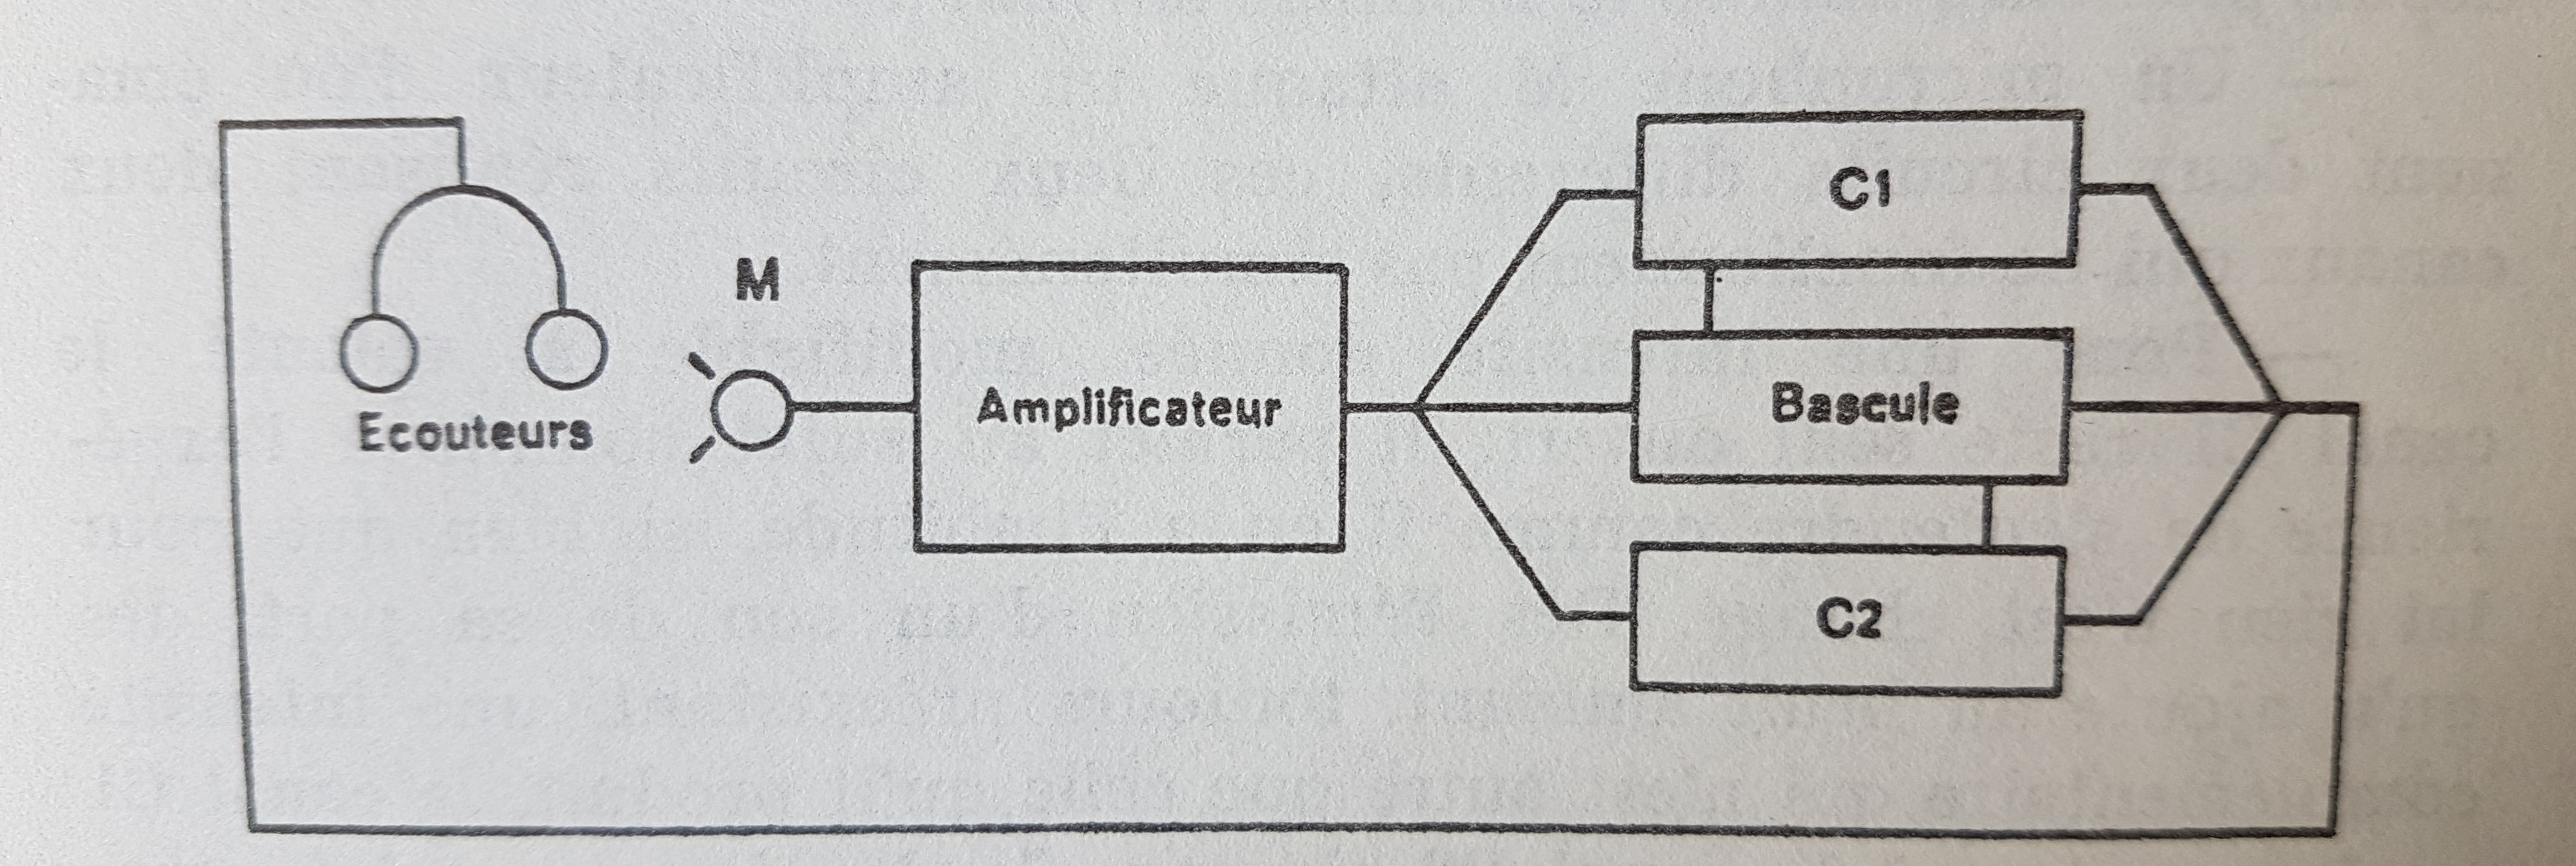
\includegraphics[width=0.7\linewidth]{images/oreilleelectro.jpg}
	\caption[oreilleelectro]{Schéma initial de l'Oreille
          Electronique}
       
	\label{oreilleelectro}
\end{figure}


      
En fait, ce schéma comprend le\textit{ feed-back}, un des principes
cybernétiques lié au concept de l'\textit{homéostasie} tel
mentonné dans le dictionnaire de psychologie.\autocite[298]{doronparot}\footnote{Doron et Parot, rétroaction;
  feedback positif = il faut varier, f.négatif= ne rien faire,  feed-back, Doron/ Parot, .p177 : cybernétique. Concept de l'homéostasie, Cannon}



 En effet, dès les premières
séances, Tomatis constate une amélioration temporaire de la voix, se
stabilisant avec l'entraînement, et établissant ainsi
\textbf{le lien frappant entre l'écoute et
  l'émission vocale}.

\textbf{L'ensemble de ces considérations préalables nous permettent d'accéder au choix de
cette méthode de testing appliquable à notre recherche.}
 
%\chapter{Alfred Tomatis}


\section{Le test d'écoute de Tomatis}


Selon son ouvrage,\footnote{\emph{Éducation et
    Dyslexie}\autocite{tomatis:education}}la représentation graphique tirée du 
 ``\emph{Hearing Test}'' distingue l'écoute générale de l'auto-écoute avec l'observation des modifications et des évolutions des courbes
  aériennes et osseuses.\footnote{<<\,Considérations sur le test d'écoute\,>>. Propos
  	recueillis au cours du \textsc{iii}\ieme\ congrès international
  	d'audio-psycho-phonologie (Anvers 1973) lors d'un entretien
        avec B. Auriol. \autocite{auriol_stress}}





Tomatis a défini la «courbe d'écoute idéale», courbe qui correspond à l'oreille absolue
des chanteurs et des musiciens,  avec  le ténor italien Enrico
Caruso (1873--1921) dont il a analysa la voix à partir des
enregistrements sur disque. Caruso représentait la courbe auditive
optimale dont il décida de se référer. C'est une courbe ascendante entre 500 et 2000
Hz qui correspond à une pente d\textquoteright environ 6 à 18 db/octave,
puis un dôme entre 2000 et 4000 Hz et ensuite une légère descente. 

      Sur le plan de la physique pure, elle indique les réponses de l'oreille
lorsque celle-ci fonctionne bien. Elle répond en fait à la courbe
de Wegel dite ``courbe en citron", inversée.\footnote{
		Voir l'annexe \ref{acoustique} p. \pageref{acoustique}
		 pour cette partie technique.}.

               

L'acquisition de cette courbe idéale correspond à l'\textsl{harmonisation}
du jeu de deux muscles de l'oreille moyenne. Celui-ci 
permet de régler en permanence la pression interne au niveau du
labyrinthe.

Sur le plan du test d'écoute, on évaluera et visualisera la différence
graphique selon la courbe dite 
idéale. Lorsque la forme de
courbes est continue et parallèle et qu'il n'y a pas de distorsions, on parle d'harmonie. L'harmonie
est la représentation de la régulation des émotions, l'équilibre entre
une écoute
intérieure et extérieure.

Ces paramètres sont importants et nous reviendrons plus en détail sur
la passation du test d'écoute.
%\enquote{\emph{L'oreille a un
%psychisme\autocite[{tomatis:loreille}.}} 

Lorsque l'interprétation des informations transmises à l'oreille est
erronée, il y a une 
\textbf{distorsion d'écoute}, liée au dysfonctionnement
de ces deux muscles dont le rôle est de permettre l'arrivée
harmonieuse du son dans l'oreille interne, puis au cerveau. Car, lorsque
le message sensoriel est altéré, le cerveau se protège en déclenchant
des mécanismes d'inhibition de l'écoute, traduit souvent par un relâchement de
ces plus petits muscles du corps humain. Ce potentiel acquis à
la naissance peut s'altérer avec les difficultés inhérentes à
la vie et la protection recherchée (inconsciemment) contre certaines agressions et le subterfuge le plus
efficace qu'a élaboré le cerveau est
d'introduire des distorsions, comme citées plus haut. De même, constate B. Auriol
les différents maux comme l'otite, l'eczéma, l'hyper
ou hypo sécrétio de sébum sont liés à l'interaction de sons refusés
inconsciemment.  \autocite  [19--20] {auriol:cle}




Car,même si le relevé des seuils donne des résultats objectifs ---
quoique la notion d'objectivité comme dit précédemment, est très
complexe avec le son ---il peut paraître paradoxal de pouvoir détecter
le potentiel d'écoute pour chaque patient en particulier.  En fait,
selon les désirs du patient de se servir des sons qu'il a à sa
disposition, celui-ci choisira d'en entendre seulement une partie. Il
est en vérité \textit{capable physiquement} de les entendre mais ne
les veut pas psychologiquement. Le cerveau a le pouvoir d'assourdir
certaines fréquences, de les masquer jusqu'à les faire disparaître peu
à peu de son champ d'écoute. Les zones corticales, qui se chargent de
l'intégration sonore et de l'écoute sélective, sont sollicitées par
des impulsions électriques mais aussi par une forte irrigation
sanguine et jouent ce rôle de protection.  \autocite [14] {auriol:cle}
Car par réflexe d'auto-défense, de ``survie'', les sons sont en
quelque sorte annihilés alors que l'oreille peut les collecter. Le
cerveau crée ainsi des\textbf{ distorsions d'écoute}
\autocite{tomatis:education}.

  



  




 




  


Pour aller plus avant dans le noyau du thème abordé, nous considérons utile
l'approfondissement de certaines notions. La crédibilité d'un test passe aussi dans la crédibilité des 
notions scientifiques qui la soutiennent, raison pour laquelle nous allons expliquer brièvement  la 
méthode Tomatis avec son test d'écoute mais aussi la
divergence d'opinion entre von Békésy et Tomatis, c. à. dire leurs différences conceptuelles de la 
physiologie auditive. 
\section{Méthode et test d'écoute}

Par {\textit{l'audio-psycho-phonologie}}, on entend l'étude des
phénomènes auditifs, phoniques et psychologiques et leurs anomalies.
De ces dernières,  dérive la mise en place d'un processus pédagogique
et/ou thérapeutique pouvant
utiliser plusieurs techniques.
Une de ces techniques,
  appelée
\label{outil_oreille_electro}
\textit{Oreille Electronique}, utilise
un système appelé \textit{ la
bascule} \autocite{escera-key},comme déjà cité plus haut (Cf. 3.1) permettant de créer une alternance 
entre deux conditions perceptives
du même message sonore, avec un passage soudain et imprévu de fréquences graves à des
fréquences aiguës.
Cette application favorise une amélioration naturelle \emph{d'interprétation du message
sensoriel}, répondant à des objectifs rééducatifs, par ailleurs en
interaction avec la psycho-neuro-immunologie (\gls{PNI})\footnote{Cf. Glossaire.}, elle-même sensible à
l'impact des événements psychiques sur le système immunitaire.
Cette conception intégrative de l'homme met en interaction toutes les
dimensions corporelles et psychologiques, dont les émotions et les cognitions.
``L'effet Tomatis''  est constitué des principes suivants:
\begin{itemize}
	\item La voix est soumise à l'oreille, c'est-à-dire la voix ne contient que ce que l'oreille entend.
	\item Toute modification de l'audition implique immédiatement
          et inconsciemment une
          modification de la voix.
	\item Il est possible de transformer l'émission vocale par une stimulation
auditive
		entretenue pendant un certain temps (loi de
               ``\gls{rémanence}'')\footnote{Cf. Glossaire.}.
%   \begin{enumerate}
%\item lualatex master
%\item makeglossaries master)
%\item lualatex master
%\end{enumerate}

\end{itemize}
Dans sa globalité, l'``effet Tomatis'', qui met en rapport audition et phonation, se manifeste par une 
action
simultanée sur les fonctions de
l'oreille en touchant le système nerveux central (SNC) (coordination
                motrice et équilibre), par l'intermédaire du système
                vestibulaire.
                De même, cet ``effet Tomatis'' agit aussi sur certains troubles
                neurophysiologiques et  joue un rôle de dynamisation cérébrale et corporelle
                par des fréquences spécifiques.


%Il est important d'offrir une vision plus ample de
Voyons à présent l'articulation entre la théorie de von Bekésy et celle de Tomatis.
%raison pour laquelle nous présenterons les différences conceptuelles de
%base entre les deux chercheurs.
En effet, le concept Tomatis prouve le bien-fondé du choix de ce test. Il est l'un des aboutissements de
ses recherches car, puisant  ses racines dans l'audiologie, il s'en
démarque toutefois pour les raisons que nous allons voir succinctement.

\section{Evolution des hypothèses inhérentes au système d'écoute}
Pour une meilleure compréhension des différences conceptuelles de von Békésy et Tomatis, nous 
verrons que de nombreuses  hypothèses ont été élaborées au fil du temps et que le sujet reste 
d'actualité que ce soit sur la cochlée ou  la physiologie auditive. %L'hypothèse soutenue par 
%Tomatis  avait 
%déjà été évoquée en 1863 par Von Helmholtz. 
Ainsi, dans la chronologie des découvertes scientifiques,  l'hypothèse de la \textbf{``batterie de
	résonateurs''}  de Von Helmholtz (1863)  a été remplacée par la
théorie dite de  --- ``l'onde propagée'' --- ou --- ``des
tourbillons'' ---  de Bekésy (1928).
Cependant, relate l'auteur de cette recherche \autocite[p 24---28]{auriol:cle}, les travaux de Leipp (1970, 
1976), Tomatis (1972), Sellick 
et coll.,(1982), Wilson (1983),
Johnstone (1986), Dancer et
Franke (1987) ont revalidé la position de Von Helmholtz.

\paragraph{Les différences conceptuelles de la physiologie auditive
  entre Bekésy et Tomatis}




En bref, dans  l'approche de von \textbf{ Bekésy} (Budapest 1899 -- Honolulu 1972,
physicien américain d'origine hongroise) ses
recherches en acoustique concernant les techniques de communication
téléphonique l'amenèrent à s'intéresser au problème de l'audition et à
élaborer des modèles de fonctionnement de l'oreille. Il élucida en
particulier le rôle de la membrane basilaire, et ses découvertes
permirent d'améliorer les traitements de la surdité (PN, prix
Nobel de physiologie 1961).
Sa vision affirme que la fonction principale de l'oreille 
consiste à transmettre les sons de manière \textbf{passive} au même titre qu'un micro et le rôle des 
osselets
est limité à la simple transmission du
son. En d'autres termes, le son emprunte pour son passage un pont  constitué du marteau, de l'enclume 
et de l'étrier. Il avait déjà énoncé cette loi en 1923, et elle a été adoptée
universellement dans la physiologie humaine.

En divergence avec von Békésy, \textbf{Tomatis} oppose la conception de la
physiologie auditive comme \textbf{active} et non
passive.\footnote{Cf. Annexe A. 1. 1. Anatomie de l'oreille et sa physiologie}
Son originalité réside ainsi dans la transmission du son
au niveau de l'oreille moyenne et interne. Le son est conduit immédiatement en direction de l'oreille 
interne grâce à l'os périphérique qui entoure la membrane tympanique.

\begin{quotation}
	``Le tympan se met dans un certain état de tension pour jouer le
	rôle d'un diapason qui fait vibrer toute la boîte crânienne
	par l'intermédiaire du \emph{sulcus tympani}.
	\emph{C'est toute la boîte crânienne qui vibre et qui transmet le son à
		la vésicule labyrinthique et non à la chaîne ossiculaire que l'on a l'habitude
		de considérer comme le véhicule du son.} La chaîne ossiculaire est un ensemble
	qui
	joue le rôle d'\textbf{adaptateur, de régulateur et non de transmetteur}.'' \autocite {tomatis_conf1972}

\end{quotation}
\enquote {	La cochlée, de par sa grande densité, capte les sons
	et résonne comme du cristal.}  \autocite {tomatis_conf1972}
Notons que la transmission du son par l'os est extrêmement rapide, de
5000 $m/s$.

De plus, le \textbf{tympan}, dans son rôle de transmetteur dans l'oreille
          moyenne, effectue --grâce aux muscles de l'étrier et du marteau--
		un\textbf{ travail de visée} en ciblant les sons. Il
se tend
		pour se mettre en résonance avec les sons à percevoir.
               Il fait aussi un autre travail qui est celui de \textbf{sélectionner des
sons
		pour se protéger}. Ainsi le tympan se tend et se détend,
              amortit et adapte
l'intensité
		sonore inondant  l'oreille interne.
		
		
Cette sélection pour se  protéger rejoint et consolide ce que nous évoquions plus haut à propos des 
distorsions et du pouvoir protecteur du cerveau.
En ce qui concerne notre sujet, le passage des sons différencie donc les deux conceptions énoncées 
mettant aussi en lumière  le rôle d'adaptation des tourbillons et non de transmission, 
d'où l'importance de  
la conduction osseuse, relatée et référée dans son test d'écoute.

%Cette hypothèse de Tomatis semble s'ajuster actuellement avec celle 

%On pourrait aussi rajouter  l'analyse
 %        fréquentielle que fait Tomatis au niveau de la\textbf{ cochlée}:
%l'onde acoustique arrivant par le canal auditif
%jusqu'au tympan  excite la membrane tympanique, donc l'os de la caisse
%du tympan \autocite {tomatis_conf1972}.%auriol:cle
%\enquote {A l'instar d'une
%peau de tambour qui fait chanter le bois auquel elle est attachée,
%c'est toute la boîte crânienne qui est inondée de sons et en particulier
%l'oreille interne. La cochlée, de par sa grande densité, capte les sons
%et résonne comme du cristal.} Notons bien que la transmission du son par l'os est de
%5000 $m/s$.
%Les fréquences qui forment les sons vont ainsi exciter les cellules
%ciliées la tapissant, tel un piano enroulé.
%Chaque fréquence se dirige \textbf{instantanément }et
%naturellement vers la cellule ciliée correspondante grâce à la
%forme du limaçon, produisant ainsi un tri fréquentiel
%instantané.
\begin{figure}
	\centering
	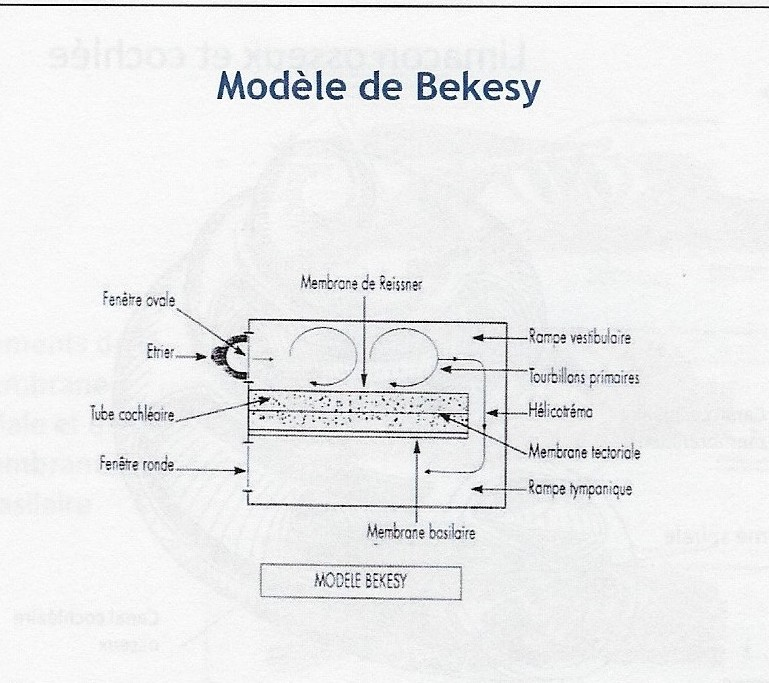
\includegraphics[width=1.0\linewidth]{images/Cochleederoule_bas.jpg}
	\caption[Modèle de Békésy]{Cochlée selon Békésy/ Tomatis Développement SA, 2012}
	\label{fig:cochleederoulebas}
\end{figure}

\begin{figure}
	\centering
	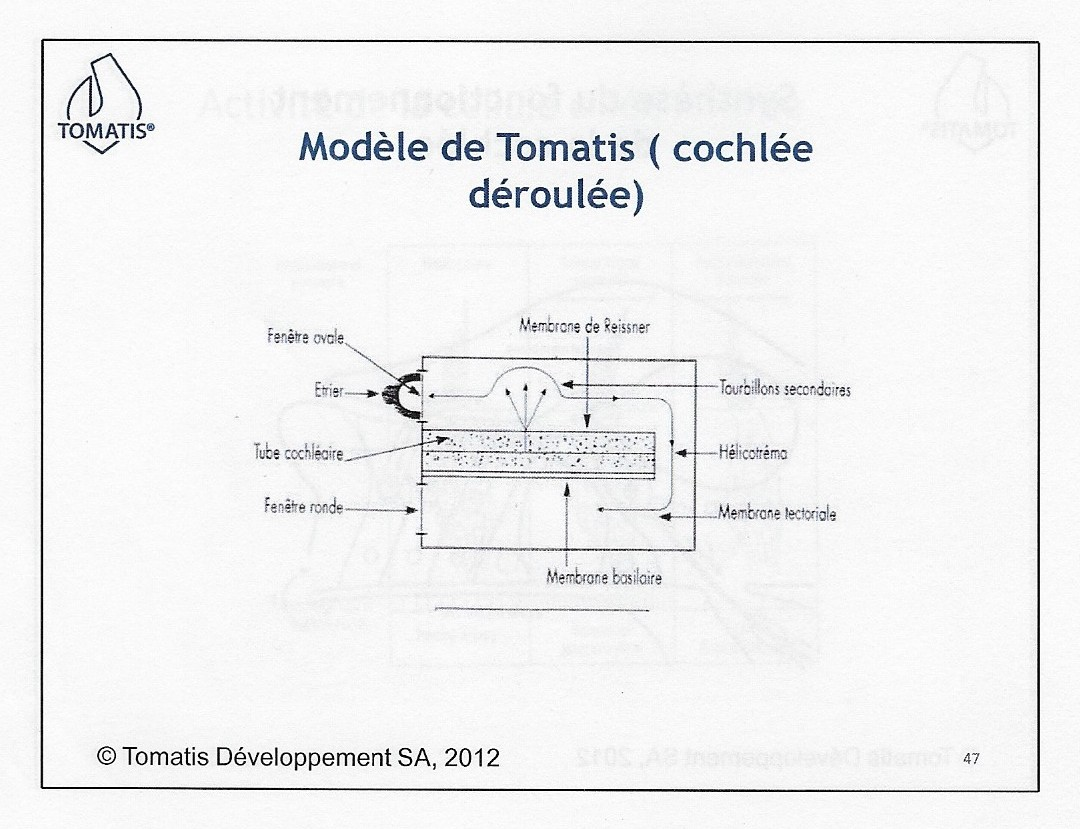
\includegraphics[width=1.0\linewidth]{images/Cochleederoule_haut.jpg}
	\caption[Cochlée selon Tomatis]{Cochlée selon Tomatis}
	\label{fig:cochleederoulehaut}
\end{figure}
%, dans un entretien (2012),
%réalisé par Laurent Salters et Vincent Gaullier, basé sur la revue
%\textit{``Look at science''}\,>>}
%Le rôle des tourbillons est de \textbf{s'adapter aux bruits}
%et non de transmettre les sons.
%Lorsque l'intensité des sons aug\-men\-te,
%l'ex\-ci\-ta\-tion des cellules ciliées provoque des perturbations liquidiennes
%dans l'oreille interne, c'est-à-dire des tourbillons. Ceux-ci se propagent
%et sont amortis par l'étrier. Si les sons atteignent une intensité
%dangereuse pour les cellules ciliées, l'étrier réagit fortement et
%entraîne une réaction du marteau qui modifie la tension du tympan.
%A son tour, le tympan, relâché, amortit le volume sonore transmis
%à l'oreille interne, comme la paupière qui se ferme quand la lumière
%est trop intense.
Par ce rapide survol, nous constatons que  le 
chemin 
parcouru par 
le son s'explique avec différentes théories  dont celles de von Békésy et 
Tomatis, que l'énigme du rôle de la \textbf{cochlée}  persiste, l'audition restant  encore sujet de grandes 
recherches dont celles menée par Christine Petit  et son équipe (2012, 
2019)%Même si le rôle de la cochlée reste encore mystérieux, 
qui relève que 
\nomenclature{cochlée}{Anatomie : organe de l'audition, appareil sensoriel,
	en forme de spirale, la cochlée, incluse dans l'os du rocher,
	forme le limaçon membraneux, se situe dans l'oreille interne et
	permet de déceler des sons extrêmement faibles, de discriminer des fréquences
	et de masquer des sons faibles par des sons forts.}
<<\,c'est une sorte de minuscule appareil électroacoustique capable
de discréminer des sons extrêmement faibles, capable de \emph{masquer
	les sons faibles par des sons forts}, pouvant \textbf{distordre les
	sons,} et \emph{capable d'élaborer un traitement extrêmement
	sophistiqué des sons} ``. \,>> \autocite{petit_lookscience}   \footnote{Christine Petit, titulaire de la 
	chaire Génétique et
	Physiologie cellulaire au Collège de France}


 




%Somme toute, on peut penser que Tomatis a été très à l'avant-garde
%dans ses recherches.

%D'autres études récentes prouvent l'effet anxiolytique lors de
%l'application de cette
%méthode Tomatis\footnote{\emph{Tomatis Research and Publication} www.tomatisassociation.org}  avec Flehming
%I., 1996 \footnote{Dr. med. Inge Flehming,
%	neurologue, neuropédiatre \emph{``Grundsatz-Gutachten zur Behandlungsmethode
%		nach Prof. Tomatis''}. Voir
%\href{http://www.analytische-hoertherapie.de/uploads/tx\_templavoila/Grundsatzgu
%tachten\_zur\_Behandlungsmethode\_nach\_Prof.\_Tomatis.pdf}{le site
%web.}} et Du Plessis W. F. and Van Jaarsveld P. E., 1988.
% \footnote{Du Plessis W. F. and Van Jaarsveld P. E. ,1988, \textit{``Troubles
%psychologiques''} (Université de Potchefstroon
%- Afrique du Sud).
	%\textit{``Audio-psycho-phonology : A comparative outcome study on anxious
%primary school pupils'''},  Afr. Tydskr. Sielk. 19818 (4) 144--151. Du Plessis, W.F., Burger, S. (2001) [\ldots]
%	\emph{A pilot study involving the Tomatis method.}, Sud Africa J.
%Psychol.}

\section{Technique de passation du test Tomatis}
L'appareil de Tomatis, basé sur la reconnaissance des sons purs et
permettant d'objectiver la qualité de l'écoute
 a été créé dans les années 50, comportant un générateur de fréquences
 (avec
 des sons
  purs de \SIrange{125}{8000}{\Hz}, d'octave en octave, en passant par les valeurs
\SIlist{1500;3000;6000}{\Hz}, et dont l'intensité peut varier de 5 en \SI{5}{\dB}, de \SIrange{10}{100}{\dB}.)
Ces derniers sont propagés par une
  transmission aérienne avec un casque, et par une propagation osseuse
  avec un vibrateur.

  L'identification de ces sons est 
  signalée par la levée de la main homolatérale (droite, gauche ou
  bilatérale).
Un volume initial très faible est suivi d'une intensité
progressive jusqu'à la manifestation d'une réponse gestuelle.
 
Nous allons développer à l'aide de la représentation
graphique ci-dessous,  les paramètres du\textbf{ seuil}, de la
\textbf{spatialisation}, de la \textbf{sélectivité} et de l'\textbf{audiolatérométrie}.


\begin{figure}
	\centering
	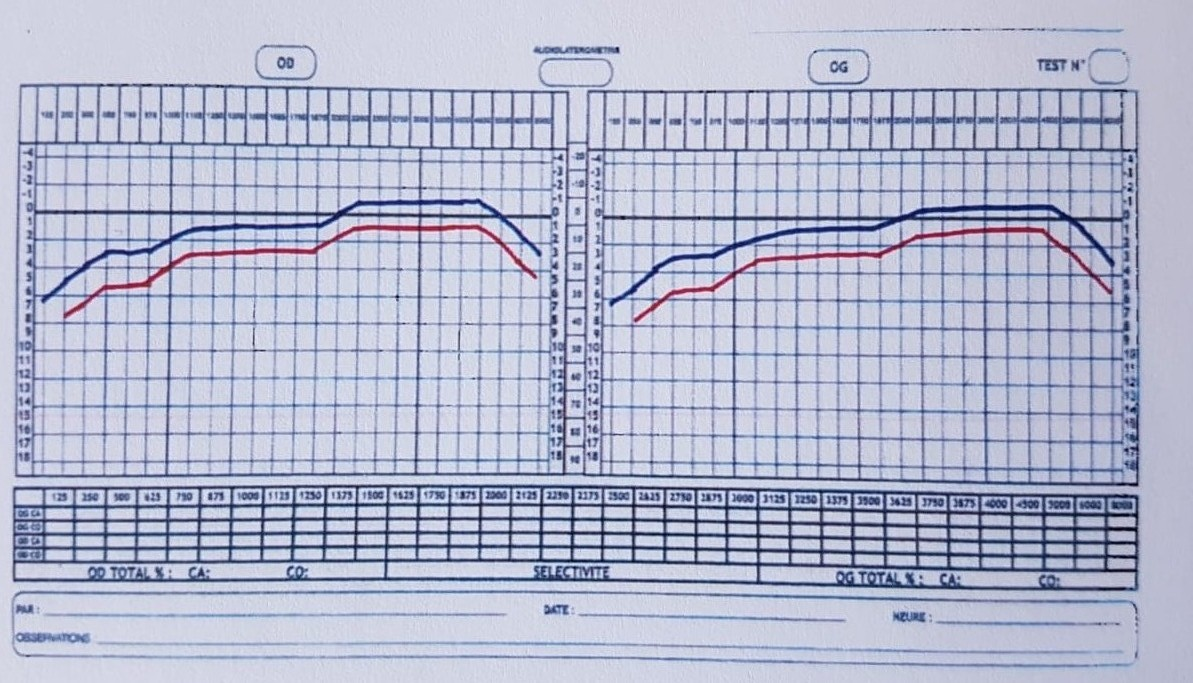
\includegraphics[width=0.7\linewidth]{images/courbeideale.jpg}
	\caption{Diagrammes des courbes relatives à l'oreille droite et
          gauche; tracé bleu: c. aérienne; tracé rouge: c.
          osseuse, (Copyrights Tomatis Développement S.A.  2014) }
	\label{fig:courbeideale}
\end{figure}




\subsection{Identification des seuils auditifs individuels}

Cette \textbf{détection}, destinée à relever les deux profils d'écoute
en vue d'une application thérapeutique, 
s'effectue, d'une part, à l'aide d'une
conduction aérienne par \textbf{écouteurs}, où l'oreille interne
informe le nerf auditif,  et d'autre part, à l'aide
d'une conduction osseuse par\textbf{ vibrateur}, excitant le crâne au
niveau de l'
\textit{os mastoïde} transmettant à son tour à  la voie nerveuse
auditive.

\subsection{Représentation graphique}

Parmi les quelques éléments différentiels
apparaissant par la suite dans les observations cliniques, il est utile de retenir
que le seuil d'écoute est représenté par un point, résultant entre la
fréquence (abcisse) --spectre couvrant 20
fréquences (de 125 à 8000 Hz)--   et le volume
(ordonnée) dont chaque carré représente une différence de \SI{5}{\dB} en
volume, partant de dB de $-20$ à 90 dB.


Les points reliés dessinent deux courbes caractéristiques, (aérienne
et osseuse), permettant de relever les paramètres d'harmonie ou
          d'équilibre, ceci 
 	en comparaison avec la courbe idéale : on parlera
        d'équilibre ou de
 	déséquilibre, d'harmonie ou de dysharmonie.
        
        \begin{enumerate}
 
  \item   les seuils d'écoute sont reconnaissables par des points au niveau de 
          chaque fréquence émise et selon le volume entendu par le
          patient. Les points reliés créent les deux courbes.
 	\item le son : son pur en 20 fréquences différentes, de 125 à 8000 Hz.   
 	\item le volume: dB de $-20$ à 90; un carré sur le graphique représente une différence de \SI{5}{\dB} en
 		volume 
 	\item la courbe: est le résultat des points reliés des seuils
          d'écoute; ils 
          dessinent deux courbes caractéristiques, l'une aérienne et l'autre osseuse.
          L'observation des courbes d'écoute relevées vont permettre
          de les classer selon les paramètres d'harmonie ou
          d'équilibre, ceci 
 	en comparaison avec la courbe dite idéale : on parlera
        d'équilibre ou de
 	déséquilibre, d'harmonie ou de dysharmonie
        
      \item L'équilibre/déséquilibre graphique s'observe 
        -entre les deux oreilles, l'oreille droite et l'oreille gauche
        et 
        -entre les deux courbes aériennes et osseuses,
        
        dont les 
        croisements, les pics ou les échancrures notifient 
        l'écart en 
        qualifiant l'écoute d'harmonieuse ou de
        déséquilibrée. 
      \end{enumerate}
      
 En  conséquence,  s'il y a une modification
          graphique des courbes, elle 
          permet d'évaluer la transformation de l'écoute pré-et
          post -thérapie.
          

 
 







\paragraph{Remarque}


Tomatis a volontairement décalé les étalonnages des deux courbes (aérienne
	et osseuse) pour pouvoir distinguer les différentes réponses et interpréter
	les distorsions. Lorsque l'écoute est parfaite, les
	courbes aérienne et osseuse se confondent mais pour l'analyse des
	résultats, on a déterminé des courbes parallèles, la courbe aérienne
	devant être au dessus de la courbe osseuse.


\begin{figure}
	\centering
	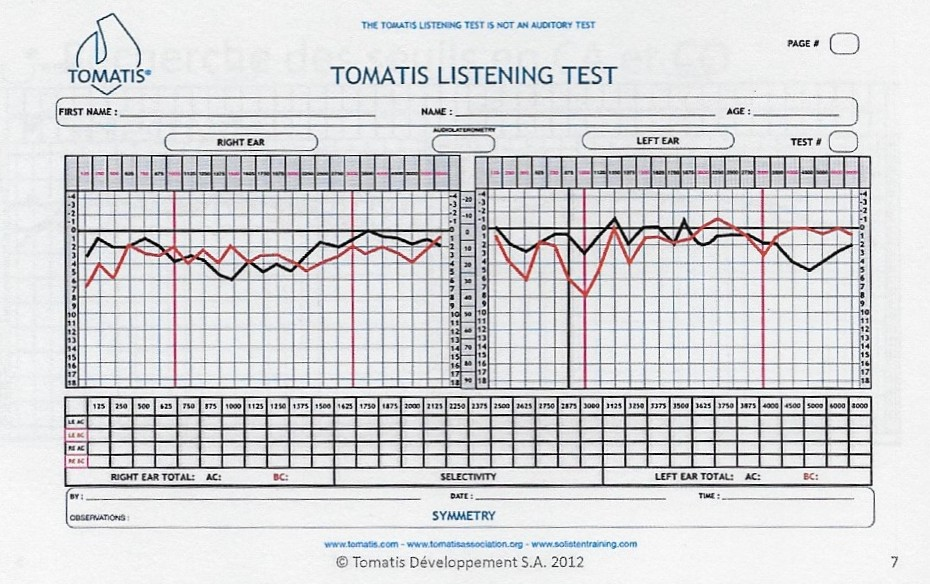
\includegraphics[width=0.7\linewidth]{images/tomatisListeningTest.jpg}
	\caption[Graphique du test d'écoute]{Graphique du test
          d'écoute d. + g. incluant, en bas, le test de sélectivité}
	\label{fig:tomatislisteningtest}
\end{figure}


\paragraph{Les seuils auditifs en priorité:} 
nous donnerons la priorité à la comparaison 
des seuils auditifs de la courbe aérienne et osseuse ainsi que leur impact sur les 3 zones,
 raison pour laquelle nous passserons brièvement en revue les
différentes techniques d'observation telles la
spatialisation, la
sélectivité et l'audiolatérométrie.
\footnote{ Il serait intéressant d'englober toutes ces observations, 
  mais ceci dépasserait le cadre de notre étude. Toutefois, à propos des seuils
  auditifs, nous nous sommes référés à  
l'étude effectuée par le CNRS de Montpellier citée plus haut.}


\subsection{La spatialisation}

  


En relevant les seuils on assiste à la capacité 
d'\textbf{identification} et de \textbf{localisation} de la
\textbf{source sonore} comportant parfois des confusions et/ou des inversions
latérales.

La \textbf{spatialisation}
indique le degré d'élaboration de la latéralité auditive,
et elle fournit des repères sur la façon dont le cortex intègre les informations
par les faisceaux homo et hétéro-latéraux fonctionnellement différenciés.(cf.annexes?????)
Les erreurs de spatialisation peuvent refléter la confusion
de l'intégration corticale des informations et traduire une latence/
incertitude de localisation de la provenance du son.
(Tomatis souligne, dans son expérience, que la difficulté du sujet à en déterminer la provenance relève d'une mauvaise coordination, d'un manque de confiance en soi ou
d'une mauvaise organisation des idées.)??????


\subsection{La sélectivité}

  
  La \textbf{sélectivité }s'assimile  à  la capacité d'analyse tonale,\textquote{faculté que possède une oreille de percevoir
une variation de fréquences à l'intérieur d'un spectre sonore, et
de situer le sens de cette variation}\autocite{tomatis:loreille} dont 
le but est de déceler l'ouverture ou la fermeture de cette
caractéristique auditive. Cette dernière permettant de donner des informations sur la
qualité d'écoute, touchant aux aspects  linguistiques (conscience
phonémique), cognitifs ( fonctions exécutives) et émotionnels action
efférente, présence d'anxiété).
Le langage étant lui-même constitué de milliers de phonèmes, on reconnaît les possibilités auditives du patient si celui-ci  distingue au minimum la différence d'un son ``pur" d'une octave à l'autre.  


\subsection{ L'audiolatérométrie}
  
Grâce à l'\textbf{ audiolatérométrie} on définit  la latéralité droite ou gauche du patient. La dominance
de l'oreille droite comme oreille directrice doit être manifeste car
selon ses travaux, il y a une différenciation fonctionnelle
physiologique due à la longueur des nerfs récurrents. 
Si le cerveau préfère prendre l'oreille droite comme
``directrice'', c'est que le trajet emprunté par l'oreille droite au cerveau est plus
court;
ainsi
les informations circulent plus rapidement jusqu'à l'hémisphère gauche.


      



 
Ainsi, après la passation du test d\textquoteright écoute, nous nous
trouvons en présence de deux grilles contenant chacune deux courbes,
en général, de deux couleurs différentes complétées par l'indication
des inversions ou confusions de sons, par des données sur la sélectivité
et en même temps par des chiffres qui correspondent à l'épreuve d'audiolatérométrie.
Les résultats du test permettront de faire une comparaison avec la
courbe idéale.


\subsection{Les trois zones du test d'écoute }
Sur le le graphique du test, les fréquences observées vont être partagée en
trois, permettant la mise en évidence de différentes zones à l\textquoteright intérieur
de chaque diagramme. Les fréquences se répartissent des 
graves aux aigues, de la façon suivante :
\begin{itemize}
\item Zone 1 : de 125 à 1000 Hz : les graves, la zone vestibulaire
\item Zone 2 : de 1000 à 3000 Hz : les mediums, la zone du langage
\item Zone 3 : de 3000 à 8000 Hz : les aigus, zone cochléaire
\end{itemize}
Ces différentes bandes sonores nous donneront des éléments
d'interprétation.
Nous nous appuyons ici sur les affirmations expérimentales de Tomatis.


\section {Analyse et interprétation du test}


De manière générale, l'interprétation du test insiste sur le relevé graphique
des
courbes et accorde des
significations différentes aux zones spectrales.
\footnote{ Ces données interprétatives sont fiables, confirmées par
  les recherches de Tomatis dans le domaine
  empirique.}

Ce sont des comparaisons graphiques des courbes. 
On considère l'allure générale des courbes, on compare leur dessin
: la forme des courbes, l' équilibre, la symétrie ; et on étudie leurs
rapports entre eux : 

courbe aérienne (CA) - courbe osseuse (CO) - rapport entre CA et CO
pour chaque oreille - rapport entre CA et CO d\textquoteright une
oreille à l'autre. si ce rapport est correct, CA est placée au-dessus
de CO sur la grille.


\subparagraph{Les deux types de courbes véhiculent chacune des informations spécifiques
sur la posture d'écoute du sujet : }
\begin{itemize}
\item La conduction aérienne : traduit la vie sociale, la manière de communiquer
et de s'extérioriser
\item La conduction osseuse : traduit la vie intérieure, mode de fonctionnement
organique, d'une façon générale : liée aux tensions. C'est la courbe
de l\textquoteright auto-écoute, de l\textquoteright auto-contrôle,
de l'écoute intérieure.
\end{itemize}

\subparagraph{Les courbes donnent des informations selon leur ascendance, leur
continuité et leur similarité oreille droite/ oreille gauche.}
\begin{itemize}
\item Continuité de la courbe : Si une courbe est continue, elle définie
comme harmonieuse et ne comporte pas de pics, de scotomes (échancrure)
qui laisseraient
supposer l'existence de nombreuse tensions.
\end{itemize}
Situées en CO, ce sont des tensions internes non exprimées : attitude
calme mais très tendue intérieurement.

Situées en CA, ce sont des tensions réelles et exprimées au quotidien
: soit somatisées, soit verbalisées ou soit manifestées sur le plan
affectif (pleurs).

\subparagraph{Les trois zones du test d'écoute : }
\begin{itemize}
\item Zone 1 : de 125 à 1000 Hz : les graves, la zone vestibulaire, élaboration
du schéma corporel, des repères temporo-spatiaux, adresse motrice,
esprit pratique.
\item Zone 2 : de 1000 à 3000 Hz : les mediums, la zone du langage, de la
verbalisation, compréhension, mémorisation, de l'intégration des lois/
des règles, esprit analytique.
\item Zone 3 : de 3000 à 8000 Hz : les aigus, zone cochléaire, de l'énergie,
de l'imagination, de l'expression, motivation, esprit synthétique.
\end{itemize}

\subparagraph{Les trois zones de fréquences du test d'écoute correspondent à des
caractéristiques précises ; et, avec l'allure des courbes, on doit
tenir compte de leurs particularités.}

Lorsqu'une zone du test d'écoute est nettement dominante et semble
traduire une caractéristique de la personnalité, on peut situer un
sujet dans un registre particulier correspondant à son tempérament.

\begin{itemize}
	\item courbe accentuée dans la zone fréquentielle des graves : tempérament
	orienté vers le corps,
	
	\item courbe accentuée dans la zone fréquentielle des médiums : tempérament
	paranoïde, attaché à la logique, la règle, le raisonnement 
	
	\item courbe accentuée dans la zone fréquentielle des aigus : tempérament
	schizoïde, reflétant une recherche de créativité. 
\end{itemize}


La simplicité de
passation pour le test d'écoute et 
 l'évaluation des indices de réception évitent toute confusion
à l'aide de réponses gestuelles.



 







\chapter{Etude avec utilisation du test Tomatis en clinique psychiatrique.}
Nous savons que la musicothérapie est de plus en plus intégrée dans
les milieux psychiatriques. Nous avons choisi ce terrain d'étude car 
nous  travaillons dans ce domaine  à temps partiel comme musicothérapeute.
\section{Cadre de travail}
 La Privatklinik
de Meiringen est  spécialisée en
addictologie dans le canton de Berne. Elle dispose d'une capacité de 195 lits, 33 médecins et
psychologues, secondés par 177 soignants qui assurent le suivi du
patient. Regula Lehman, musicothérapeute à temps complet, et nous-même avons
collaboré  pour l'organisation de la mise en place de l'étude. Celle-ci porte sur un même type de
population dans le contexte et cadre  précis d'une prise en charge globale
par les médecins, les psychologues, les physiothérapeutes,
ergothérapeutes et les divers ateliers de créativité proposés dans
cette clinique. Nous avons principalement travaillé avec des
pathologies comme celles du burnout, de la dépendance et de la
dépression, ceci dans une tranche d'âge de 20 à 60 ans, masculin et
féminin quasi égale. 
\section{Organisation d'étude}
Au préalable, nous avons fait circuler une
feuille d'information pour expliquer notre démarche d'évaluation sur
l'hypothèse de la transformation de l'écoute du patient lors de son
séjour en thérapie. \emph{Information für Mitwirkende an der klinischen
Studie\  "Evaluierung des aktiven Hörvermögens" }. 

\paragraph{Privatklinik von Meiringen}

Information für Mitwirkende an der klinischen Studie
« Evaluierung des aktiven Hörvermögens »


Sehr geehrte Damen und Herren,

Herzlichen Dank für Ihr Interesse an dieser Studie !

Wozu dient diese Studie und weshalb werden Sie um eine Teilnahme gebeten ?

Während Ihrem Klinikaufenthalt  in der Privatklinik von Meiringen werden Sie im Kontext 
unseres multidisziplinären Teams verschiedene Therapien besuchen, unter anderem auch die Musiktherapie. Bei der vorliegenden Studie möchten wir untersuchen, wie sich die Musiktherapie auf Ihr Zuhörvermögen auswirkt.
Musiktherapie ist eine gut erforschte Intervention im Bereich des Depressions und Burnouts, da Sie ein relativ neues Berufsfeld ist, gibt es noch viel Forschungspotential.
Das Hörtest konnte sich als ein Instrument erweisen, um die Veränderung des Gehörs des Patienten bei einer Musiktherapiebehandlung zu beweisen. Die Verbindung dieses Ansatzes mit der Musiktherapie ist noch nicht erforscht und daher soll dieser Ansatz wissenschaftlich näher untersucht werden.
Wenn Sie keine Musiktherapie besuchen aber Interesse für diese Studie haben, sind Sie herzlich eingeladen, dieses Test zu tun. Im Rahmen under MAS brauchen wir unbedingt eine Kontrollgruppe.

Wie sieht eine Teilnahme an der Studie aus ?

Die Untersuchung erfolgt sehr einfach in mehreren Schritten.
Zu Verfügung steht ein Apparat, mit dem sich spezifische Hörtests durchführen lassen.
Allgemein Verlauf des Tests :  
Sie hören einen sehr leisen Ton mit Zuhörern zu und werden ihn entweder mit der rechten  oder linken Hand  signalisieren. Das dauert ungefähr 30 Minuten.
Es wird zwei Tests geben : ein vor der Therapie und ein nach der Therapie.
Wir bitten Sie auch, eine kleine Fragebogen zu erfüllen.


Falls Sie Fragen haben, dürfen Sie sich gerne via E-Mail melden : valerie.gaillard\@gmx.ch

Wir bedanken uns herzlich für Ihre Zeit und die Teilnahme an dieser Studie.


Valérie Gaillard

 Le matériel utilisé : une table, deux chaises, l'appareil
test Hearing et les écouteurs aériens et osseux, un crayon, deux
feutres ( rouge et bleu), une feuille avec la grille de fréquences à
remplir.

ZhdK : Upgrade MAS Klinische Musiktherapie 15-17

 \section{Contact avec les patients}
 
 Regula Lehman a pu
préparer  les patients avec une explication préalable. Ensuite,
ceux-ci ont signé officiellement à chaque fois leur
accord pour cette participation  \emph{"Eine schriftliche Einbewilligung zum
Test"} avant de passer ces tests dont nous nous sommes occupées.
A Regula Lehmann  \footnote{Regula
  Lehmann, musicothérapeute  à 90\%  à la clinique de Meiringen} incombait la
prise en charge des séances en musicothérapie. Nous n'avons pas pu
toujours conserver cette configuration et nous avons dû suivre parfois
ponctuellement ou pendant le temps imparti certains patients en
musicothérapie. Par contre, le travail des tests était de notre ressort.  Nous avons organisé deux groupes, un témoin, sans
musicothérapie et un autre avec. Nous avions projeté d'en avoir
10 à chaque fois, mais ce ne fut pas simple de réunir ce
chiffre. Nous étions dépendants de leur entrée en clinique et de leur
sortie, après 4 semaines de thérapies, ce qui correspond à la durée
d'un séjour moyen dans cet établissement.


\begin{itemize}
	\item 10 patients testés, groupe A en musicothérapie : un
          premier test avant leur prise en charge en musicothérapie;
          puis un deuxième test \textdegree{} : après 4 semaines de
          clinique.
	\item 10 patients testés, groupe B de contrôle qui est un groupe sans musicothérapie,
	toujours dans le même contexte, c.à.dire la clinique, le suivi et les mêmes protocoles que l'autre groupe. Un premier test avant
	le début des autres thérapies puis un deuxième test, après 4 semaines. 
	Les tests ont été faits en avril, mai, juin, juillet, septembre et octobre 2017.
	Nous avons réalisé en tout 40 tests d'écoute Tomatis. 
	Précision importante : Pour cette étude, nous avons intentionnellement exclu la thérapie avec les musiques traitées et appliquées avec Tomatis, en nous restreignant  à ce lieu où l'application de cette forme de thérapie n'existe pas.
	Durée des tests : Chaque test Tomatis a une durée  moyenne de 50 à 60  minutes par patient. Pour chacun, nous avons donc réalisé en tout deux heures de tests d'écoute avec un entretien, et leur avons demandé en plus de remplir le questionnaire WHOQOL (20mn).
\end{itemize}

\section{Le WHOQO-Bref}

Nous avons utilisé et fait en parallèle le test WHOQO-Bref avant et
après pour avoir une variable supplémentaire pour confirmer en
parallèle supposée de l'action de la musicothérapie sur une éventuelle modification de l'écoute.  C'est une
version test de 1997 issue du Programme sur la santé mentale,
Organisation mondiale de la santé, Genève. Il y a 26 questions, que le
patient a rempli lui-même en présence du thérapeute, avant le test
d'écoute. La durée pour les remplir a varié de 8 à 10 minutes en
moyenne.  Il a eu 26 tests WHOQO-Bref.
Il y a quatre domaines testés : physique, psychologique, relations sociales et environnement.
\begin{enumerate}
	\item  Le domaine de la perception physique comprend l' activité quotidienne// la dépendance et/ou l'assistance médicale// la fatigabilité, l'énergie//la mobilité// la douleur// le sommeil// la capacité de travail//
	
		 \item Le domaine psychologique :  image de soi, apparence// ressentis positifs et négatifs// estime de soi// spiritualité, croyances personnelles, religion// mémoire et concentration, apprentissage, pensée.
		
			\item Le domaine des relations sociales : relations personnelles// soutien social// vie sexuelle.
			
			\item Le domaine de l'environnement : l'environnement domestique et  physique (pollution, bruit, trafic, climat)// la situation financière//  la liberté, la sécurité physique et morale// l'accessibilité et qualité de la santé// les opportunités de détente, loisirs et d'acquisition d'informations// le transport// 
		\end{enumerate}
		
	


 \section{Les tests d'écoute} 	
 
 \paragraph{Le test d'écoute Tomatis est une traduction graphique de l'écoute, elle permet d'objectiver la qualité de l'écoute.} 
 
  \begin{enumerate}
 	\item les seuils d'écoute
 	\item le son : dB, 
 	\item le volume de $-20$ à 90 % finesse typo: le signe moins des mathématiques.
 	\item les fréquence, de 125 à 8000.   \label{chapitre 6.2t} % mets une étiquette plus
 	% ``parlante'' stp, genre ``parametres_test_ecoute''.
 	\item la courbe, par l'observation des courbes d'écoute relevées
 	en comparaison avec la courbe dite idéale : équilibre,
 	déséquilibre, harmonie, disharmonie.  
 	\item équilibre, déséquilibre graphique entre les deux oreilles et entre les deux courbes mesurées par oreille: observation des croisements, des parallèles, des
 	écarts importants entre les courbes aériennes et osseuses\footnote{Remarque :
 		Un carré sur le graphique représente une différence de 5dB en
 		volume.}.
 	\item une modification perçue ou non comme évolutive lors des transformations graphiques de courbes
 	\item  Informations croisées avec les informations récoltées   par les 3 zones du test d'écoute: ........
 	\item une constatation de la posture d'écoute et de la qualité de
 	la voix. La voix se caractérise par son volume, son timbre, sa mélodie et son langage. 
 	
 	Nous suggérons de nous référer aux différents résultats des tests de et par la voix qui ont été faits pour tenter de déterminer un état dépressif ( Test et échelle d'Hamilton). Les chercheurs de l'université de Maryland en 2004, en émettant l'hypothèse de la modification de l'articulation vocale lors d'état dépressif ( on sait que la dépression provoque des changements  neuro-physiologiques) ont révélé lors du 168ème Congrès de la Société américaine d'acoustique, que les caractéristiques vocales se trouvaient modifiées lors de sentiments dépressifs\footnote{https://www.lci.fr/sante/et-si-on-diagnostiquait-la-depression-avec-un-test-vocal-sur-smartphone-1562728.html.}.
 		
 	
 	
 Nous pouvons faire ainsi le descriptif général de la voix d'un patient dépressif :
 	\begin{enumerate}
 		\item le volume : basse intensité
 		\item la mélodie : monotone, sans modulation
 		\item le timbre : mauvaise qualité due à une pertes des harmoniques
 		\item le langage : difficulté d'élocution
 	\end{enumerate}
 	
 		
 	
 	
 	
 	\section{Les graphiques}
 	
 	....
 	\section{Les résultats}
 	
 	....
 	
 	
 	
 \section{Les résultats et réflexions}	
Le manque de temps a été le principal facteur  réducteur
de tests valables, les départs imprévus des patients, et/ou leur
absence momentanée ( visite du psychologue, maladie, etc.). rajoutés au peu de temps de travail( 10\% )ainsi qu'à la
contingence difficile due à la distance séparant Genève du lieu de travail ( Meiringen)
: comment planifier un départ imprévu d'un patient !? il a fallu parfois
faire trois heures de route pour effectuer les tests finaux d'un ou deux
patients.
  
Par conséquent,  de nombreux tests sont restés 
incomplets et n'ont pu
être validés car ils ne remplissaient pas toutes les conditions requises.  En définitive, sur 40 tests d'écoute Tomatis et 26 tests
WHOQO-Bref, nous avons choisi de ressortir l'étude pour le groupe A de
5 patients effectifs en musicothérapie, tests complets, et le groupe
témoin B de 5 patients sur 9 effectifs, sans musicothérapie et tests
complets. 
 

  
\paragraph{Les résultats}
  
  De manière très générale, les résultats obtenus ne
  sont pas significatifs.  La prise en charge en musicothérapie a eu lieu
  une fois par semaine pendant une heure, ce qui semble trop court pour observer un changement important. Nous pourrions émettre la supposition suivante :  est-ce qu'un un travail journalier, régulier aurait été indiqué pour des résultats plus rapidement visibles avec le test?
  Est-ce qu'une immersion plus intensive en musicothérapie transformerait l'écoute des patients ? 
   En comparaison avec des
  modifications importantes de courbes des tests observées généralement  lors d' une écoute
  régulière de deux heures par jour de musique pendant 15 jours, --en référence à l'entrainement des muscles de l'oreille chez Tomatis, qui, nous le rappelons, est une pédagogie de l'écoute--, il aurait été intéressant de pouvoir faire cette étude comparative dans cette clinique. Ainsi, nous aurions pu éventuellement mettre en avant  l'absolue nécessité de créer et d'instaurer systématiquement la musicothérapie dans de nombreuses institutions mais aussi  de la développer beaucoup plus intensément  si elle est déjà existante.
  Nous sommes clairement en présence d'une ébauche d'études, avec des pistes
  suggérées. Ce travail ne peut être en aucun cas considéré comme
  quantitatif.  Nous avons ainsi pris l'option de nous tenir à une
  observation, celle de la transformation de l'écoute. Nous n'approfondirons pas l'évolution des diagnostics des différentes
  pathologies des patients.  (dépression, Burn out et dépendance.)
  
  A fortiori, relevons le cas fort intéressant  d'une patiente du groupe B( sans
  musicothérapie) : 
surprise d'apprendre par le premier test que la musique pouvait l'aider
  dans sa thérapie, celle-ci s'est mise à écouter assidûment du Mozart pendant la période de son séjour, entre le 1° test et le second test.  Les résultats
  graphiques obtenus lors de sa sortie sont clairement significatifs
  et sont en concordance avec le WHOQ-Bref. 
  ......



   
   
   
   
  \end{enumerate}







\paragraph{Hypothèse}

Est-ce possible d'évaluer un travail musicothérapeutique au moyen
d'un test d'écoute?

Est-ce que le processus d'écoute en musicothérapie améliore la capacité
d'écoute ?

Est-ce que les test auditifs avant et après la musicothérapie permettent
de visualiser l'action de la musicothérapie?

\paragraph{Y-a-t-il une modification de l'écoute du patient après une prise
en charge en musicothérapie ?}

\paragraph{Est-ce que les résultats ( = un changement dans l'écoute) d'une prise
en charge musicothérapeutique peuvent être lisibles et visibles dans
un test d'écoute Tomatis ?}

Est-ce que ces résultats sont significatifs? 

\paragraph{Est-ce que l'écoute du patient s'est modifié ? si on a pu observer
une modification, dans quel sens va -t-elle ?}

Est-ce ce test valable ? est-ce que le contexte est suffisant pour
ressortir des résultats ?







\chapter{Réflexions}


Y-a-t-il une modification de l'écoute du patient lors de séances en musicothérapie?
Est-ce visible et lisible au moyen du test d'écoute employé?
Peut-on définir et retracer un chemin sonore psychologique du patient au moyen d'un test d'écoute?


Selon les hypothèses évoquées, nous avons été amenés aux réflexions suivantes.

Nous utilisons un outil qui est le son. Nous accompagnons
le patient d'un point A pour aller au point B : que s'est -il passé
dans son écoute?
En comparant les données, nous pouvons observer des résultats visibles et tangibles 
d'une transformation de la
perception basée sur un test de reconnaissance de sons;  qui permet de visualiser une transformation psychologique
de l'écoute. 


Il y a des résultats : nous pouvons faire un constat.
Ce sont des données pouvant servir à mieux comprendre le patient
et à l'accompagner dans son cheminement thérapeutique.


\subsection{L'anamnèse et le bilan en musicothérapie}

  Avant d'amorcer une thérapie, le test effectué fournit des renseignements, toujours basés sur le son, qui seront complémentaires à l'anamnèse. Nous pouvons donc l'inclure dans un  bilan en musicothérapie.

  \
\subsubsection{La communication}


  
\begin{itemize}
  \item Les questions/réponses inhérents au 
 test d'écoute provoque le dialogue. Le patient est amené de façon
 détournée à se livrer et à évoquer des détails auxquels il
 n'aurait pas prêté attention. L'anamnèse prend donc ici un autre
 caractère puisqu'elle est complétée par le son et l'écoute.

	 La relation avec le patient est indispensable à créer pour toutes thérapies. Le test peut créer dès le premier entretien une alliance thérapeutique.
	Le test représente une procédure claire qui peut être
        considéré comme un outil utile pour instaurer un dialogue avec
        le patient et servir d' indication sur le plan du travail à
        envisager.
  \end{itemize}      
\paragraph{Le test d'écoute est une forme d'intervention
  musicothérapeutique}

Le test d'écoute est en soi une forme d'intervention
 musicothérapeutique puisqu'il 
 a deux rôles intrinsèques:

 la création d' une alliance thérapeutique et
     travail avec le son avec l'implication directe du
     patient dans le rôle de la 
     reconnaissance de sons
         Il comporte un travail immédiat avec le son en impliquant le patient
 dans le rôle actif de leur reconnaissance. Il fait faire un travail de reconnaissance de sons dans
 l'espace (repérage de fréquences selon le volume). Le patient
 participe activement en fixant son attention sur les
 sons émis par l'appareil et transmis aux écouteurs en les repérant
  puis en y
 répondant. Cette implication directe conduit le patient à créer par lui-même et de manière
 inconsciente  
 son propre espace; ce  qui permettra par là même déjà d'entamer, pour certains dumoins, leur propre
 processus thérapeutique. (40% participe à la réussite d'une
                             % thérapie,(Sandra Lutz Hochreutener)
 Il peut être perçu comme un cadre médical  rassurant par nombre de patients, jouant son rôle de soutien dans la prise en charge.
  
 
En cours de la thérapie, il peut être utile d'évaluer, tout
comme se servir lors d'un voyage d'une jauge pour estimer le chemin parcouru et celui
qui reste à faire, en cas d'interrogations, de doutes dans la façon de procéder.
En fin de thérapie, il permet d'évaluer la transformation.


\paragraph{La visibilité}

Deux aspects ressortent distinctement: la visibilité et la visualisation.

La visibilité: être visible par le son est une façon de se concrétiser extérieurement en en prenant conscience: une forme de ``comportementalisme de l'audition'' .


La visualisation: se visualiser par son chemin d'écoute.  
Ce processus de visualisation tente de matérialiser l'abstraction innée dues aux propriétés du son, l'aspect intemporel et éphémère du son entre l'écoute et la vue.
Il permet de se situer dans l'espace sonore et, en un même temps, induit une prise de conscience et de distance avec soi-même. Tout le corps, physique et psychique est impliqué (--- tendre l'oreille---) avec toutes les fonctions cognitivo-proprioceptives.


Le patient obtempère aux consignes du thérapeute, fait un choix parmi des sons précis, dialogue sur les résultats, tout ceci relève déjà d'une volonté de changement intérieur, en  éveille tout au moins cette idée de déclenchement d'un travail, initie un début de cheminement intérieur.
Être accompagné dans la lecture de son évolution sonore permet de constater un résultat qui  peut le conforter ou non dans son sentiment intérieur.
	
	D'autre part, le rôle du patient est différent dans son essence même, non pas dans le sens de "patere" souffrir et subir, mais valorisé dans celui du rôle actif qu'il peut jouer : celui-ci peut se rendre compte de sa capacité à influencer sa façon d'écouter, qu'il a une présence signifiante dans sa thérapie.  Il n'est pas passif. Bien sûr, cela peut paraître une évidence car on sait l'impact de la musique sur le corps tout entier. Mais ici on rejoint  le concept de musique intégrative déjà cité\autocite[Cf.]{vrait_musicotherapie_2018}. Le patient peut être nourri par la musique mais n'est pas "passif" et seulement l'"objet " qui bénéficie du traitement musical. Son  écoute lui appartient en propre, elle est personnelle et modifiable. S'il y a modification, il peut y avoir un changement; et le mot "changement" prend alors une connotation différente,  le mouvement est y  sous-entendu,  une démarche peut en découler, voire une évolution. 


  \section{Les instruments et leur fréquence }
 De manière très pragmatique, le test peut être
considéré comme un indicateur des zones de fréquences à
privilégier dans le travail avec le patient. Chaque instrument a une tessiture
différente avec une plage
définie de fréquence. Selon l'analyse de l'écoute du patient, le choix
d'instrument à privilégier sera plus rapide et plus sûre.

      \begin{figure}
	\centering
	\includegraphics[width=1\linewidth]{images/instrumentfréq.pdf}
	\caption[Les instruments et leurs fréquences]{Ilustration des instruments avec leurs fréquences}
       
	\label{instrumentfreq}
\end{figure}
  



\section{Graphique: Zones 1-2-3 du Test d'écoute // Musicothérapie}


        \begin{figure}
	\centering
	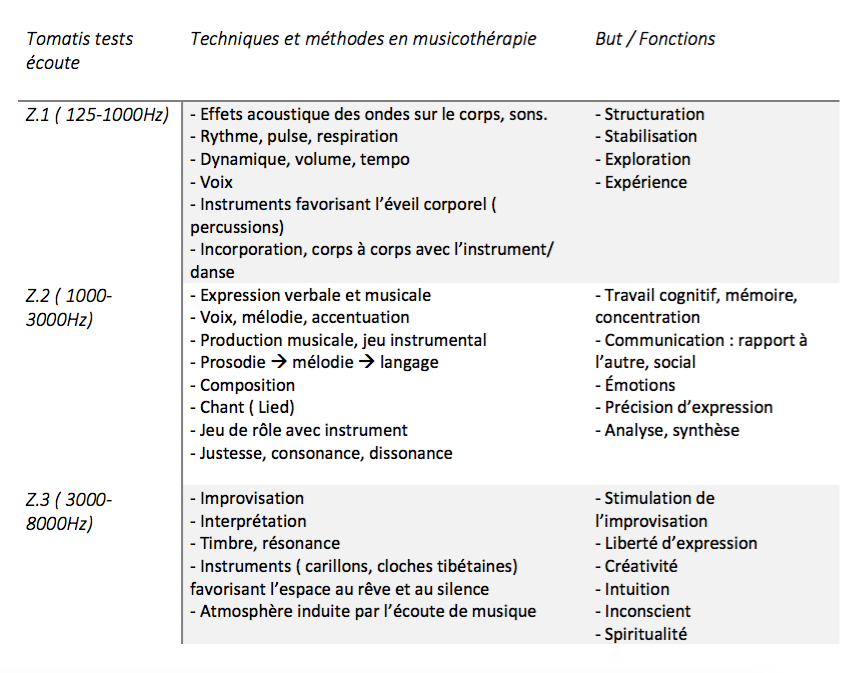
\includegraphics[width=1\linewidth]{images/testtechnmethbut}
	\caption[Zones du test avec la musicothérapie]{Schéma des
          zones avec leur application en musicothérapie}
       
	\label{testbutetfonction}
\end{figure}



S'il n'y a pas de changement visible dans le test, quelles conclusions
peut-on en tirer ? le changement va-t-il toujours de pair avec le
patient? synchronisé ou différencié dans le temps?
Comme pour toutes thérapies, le patient doit avoir le temps de l'intégrer. Quand
il aura été amené à une certaine prise de distance par rapport à
lui-même et à son environnement, il passera par différentes phases qui peuvent être celles de l'acceptation, que ce soit celle de son identité, de sa transformation, ou d'un changement dans ses habitudes --- de quitter le confort de ceux-ci même si elles sont jugées négatives par lui-même et par les autres --- . Tout ceci prend du temps et ne peut pas 
toujours  aller en simultanéité avec des résultats immédiats, avant/ après.

\subsection{Critiques: }

Par cette démarche, il y a le risque de catégoriser le patient. Les
rapports doivent rester confidentiels et en aucun cas transmis
aux assurances-maladies.
Du côté du patient, s'il est toujours en
attente de résultats, cette façon de faire peut le figer dans son parcours  Ou, au contraire, ce peut être une aide 
dans son travail, son évolution. Ces deux possibilités sont
intrinsèques à tous les tests.

Les séances de musicothérapie se sont déroulées mais  n'ont pas été
décortiquées et analysées. Ce serait passionnant de le faire mais ce n'était pas l'objectif de ce travail.		
        
 

Différents paramètres inhérents à ce type d'étude sont à
considérer. Que ce soit le manque de temps, les départs imprévus des patients, et/ou leur
absence momentanée (visite du psychologue, maladie, etc.). rajoutés à la
contingence difficile due à la distance séparant le lieu de domicile à
celui du lieu d'étude, toutes ces contingences ont été les principaux facteurs réducteurs de
tests valables.
: comment planifier un départ imprévu d'un patient !? il a fallu parfois
faire beaucoup de route pour effectuer les tests finaux d'un ou deux
patients.
  
Par conséquent,  de nombreux tests sont restés 
incomplets et n'ont pu
être validés car ils ne remplissaient pas toutes les conditions requises.  En définitive, sur 40 tests d'écoute Tomatis et 26 tests
WHOQO-Bref, nous avons choisi de ressortir l'étude pour le groupe A de
5 patients effectifs en musicothérapie, tests complets, et le groupe
témoin B de 5 patients sur 9 effectifs, sans musicothérapie et tests
complets. 
 
De manière très générale, les résultats obtenus ne
  sont pas significatifs.  La prise en charge en musicothérapie a eu lieu
  une fois par semaine pendant une heure, ce qui semble trop court pour observer un changement important. Nous pourrions émettre la supposition suivante :  est-ce qu'un un travail journalier, régulier aurait été indiqué pour des résultats plus rapidement visibles avec le test?
  Est-ce qu'une immersion plus intensive en musicothérapie transformerait l'écoute des patients ? 
   En comparaison avec des
  modifications importantes de courbes des tests observées généralement  lors d' une écoute
  régulière de deux heures par jour de musique pendant 15 jours --- en référence à l'entrainement des muscles de l'oreille chez Tomatis, qui, nous le rappelons, est une pédagogie de l'écoute --- il aurait été intéressant de pouvoir faire cette étude comparative dans cette clinique. Ainsi, nous aurions pu éventuellement mettre en avant  l'absolue nécessité de créer et d'instaurer systématiquement la musicothérapie dans de nombreuses institutions mais aussi  de la développer beaucoup plus intensément  si elle est déjà existante.
  Nous sommes clairement en présence d'une ébauche d'études, avec des pistes
  suggérées. 
  Cette étude est un mixe: quantitatif et qualitatif. Nous avons ainsi pris l'option de nous tenir à une
  observation, celle de la transformation de l'écoute.
  
 \paragraph{Un cas particulier qui mérite réflexion:}

 A fortiori, relevons le cas fort intéressant  d'une patiente du groupe B (sans
  musicothérapie) : lors du test, surprise d'abord d'apprendre, en visualisant son
  écoute, que la musique pouvait la modifier, cette patiente s'est
  mise à écouter assidûment de la musique de Mozart pendant son séjour en clinique, entre le 1° test et le second test.  Les résultats
  graphiques obtenus lors de sa sortie sont clairement significatifs
  et de plus sont en concordance avec le WHOQ-Bref!  
  Par conséquent, le test d'écoute a permis de lui faire prendre conscience d'une part que son écoute lui appartenait personnellement et d'autre part, qu'elle pouvait elle-même avoir un impact et jouer un rôle non seulement sur son écoute mais aussi sur sa propre  transformation.
Il est clair, selon Sandra Lutz Hochneutener, que la réussite d'une
thérapie réside à 40%  chez le patient.


  

\begin{itemize}
\item Est-ce que ce test pourrait être un outil pour les thérapeutes et
les patients ? 
\item Avoir un support réel, visible car graphique pourrait-il être d'une
quelconque utilité pour le thérapeute ?
\item Est-il possible, à partir de deux tests d'écoute, de tirer des hypothèses
sur l'impact du son, de la musicothérapie, du soin par le son, sur
un patient ?
\item Le patient reste au centre de nos préoccupations.
\item Serait-ce une façon de démontrer l'utilité de la musicothérapie
pour une plus large acceptation de 
cette thérapie dans plus de milieux hospitaliers ou autres ?


\end{itemize}

\section{La musicothérapie et la méthode Tomatis}

La musicothérapie et la méthode Tomatis sont des concepts très différents. Bien que la notion d'écoute les réunit, bien que leur medium soit la musique et plus particulièrement le son, d'un côté il s'agit d'une thérapie et de l'autre, il s'agit d'une pédagogie, d'un entrainement de la musculature de l'oreille. 
Tomatis se focalise et opère essentiellement sur le capteur auditif (vestibulo-cochléaire) pour amener, par ce processus, le patient à une certaine  amélioration par rapport à sa vie actuelle, à des souhaits ou à des attentes précises; celle-ci peut se réaliser au niveau du langage et ce, par l'intermédiaire de la musique et du chant. Nous pouvons de notre côté  émettre l'hypothèse que si le contrôle auditif est de bonne qualité ainsi que l'émission vocale, c'est-à-dire que la boucle phono-auditive est élaborée sans problème, l'oreille est prête, même peut-être plus prête et apte à travailler beaucoup plus en profondeur avec tous les riches moyens que la musicothérapie propose.
Préparer le terrain, faire un travail physique de fond, une
préparation de l'oreille pour que celle-ci soit totalement
opérationnelle et prête à aborder si nécessaire, un travail en
musicothérapie sur le plan physique ou psychique. simplement pour se
sentir bien sa peau, bien dans son âme.
Voilà l'hypothèse énoncée et ce que nous nous pouvons conclure, en effet.


        Est-ce utile à tout musicothérapeute d'avoir un appareil test d'écoute ? certainement pas. C'était un moyen de faire cette étude.
     Nous nous sommes  limités ici intentionnellement
     à ce concept de test.
 La matière sonore est la matière première de la  musicothérapie. 
 Par son biais, elle  apporte de multiples éléments d'évaluation du
 sujet. 
 Certains  intégrent plus que d'autres dans leur pratique des techniques relevant du domaine de la psychothérapie--de l' analytique, 
  du comportementalisme, du cognitivisme, de la  systémique ainsi que
  celles dites humanistes.  Le concept de "médium malléable" a été
  développé par  R.Rousillon\footnote{R.Rousillon,\textit{Paradoxes et situations limites,  
  		de la psychanalyse} Paris, Puf. 1991} 
  et qu'il est possible de transposer dans la matière \textit{musique} 
  pour "favoriser et accompagner le processus 
  de symbolisation"\footnote{F.X.Vrait, \textit{La musicothérapie},Ch.3, p. 112}.

 Le musicothérapeute est un être extrêment sensible avec de multiples
 ``antennes'' : l'intuition reste primordiale tout autant que  
 l'écoute. L'oreille se dresse pour une écoute empathique, pour ``rester en contact émotionnel  
 avec le patient'' , Eckert (2007) par le son qui va au plus profond de
 l'être.

 
\begin{quotation}
	\char`\"{}\textbf{``L'oreille est l'organe le plus sensible des sens 
et l'instrument de diagnostic  le plus important du
musicothérapeute.'' `\"{``Hören Musiktherapeuten anders?'' }Thomas
Stegemann, Vienne/ Seminar Zürich ZHdK, 2017.}
 	
\end{quotation}
La musicothérapie fait partie de ces thérapies dites subtiles. Elle
est très difficilement quantifiable. La
psychologie cognitivo-comportementaliste peut le quantifier avec des tests et semble avoir gagné depuis en crédibilité. Mais avec la musicothérapie ou d'autres formes de thérapie, il n'y a
jamais, à proprement parlé, d'avant et d'après mais il y a transformation.
Et les transformations échappent toujours aux quantifications. Peut-être
ici pourrons-nous apporter un outil plus objectif par un test particulier
d'écoute : la démonstration d'un travail d'écoute, d'une perception
différente, d'une sensibilité nouvelle du patient. 


% OGA: source citation Malraux

\paragraph{Apprendre à écouter}

Apprendre à écouter,
c'est un travail et des résultats pourraient être visibles.
Comme l'exprime à juste titre André Malraux : \enquote{\emph{Le monde de
	l'art n'est pas celui de l'immortalité, c'est celui de la métamorphose.}}
De même, la musique est un art produit par l'homme et qui a un impact
sur lui-même. Les deux interagissent, s'interpénètrent et s'auto-transforment
au cours des siècles.
 Ce que nous pouvons constater lors de l'aboutissement
d'une thérapie n'est pas de trouver une autre personne mais une transformation
de la perception de celle-ci par rapport au monde qui l'entoure. 
Selon
ce que nous vivons, nous nous transformons et continuons à être
soi. Nous ``sommes soi" mais autrement. Nous ne perdons
pas notre identité.


\paragraph{La musique vient dans la chair}


“La musique vient dans la chair comme un produit immatériel
qui vient travailler la zone à soigner. (...)

Je pompe de la
guérison. (...)

Depuis le début des écoutes, j’ai la sensation physique et
psychique de la
transformation. (...)

La musique est équilibrante et guérisseuse, ma zone
anesthésiée se remet à vivre, elle est remise en activité. (...)

Il y
a comme un consentement cellulaire. (...)
La béance s’estompe, cette
partie redevient comme les autres.


Apaisement. Consentement. Réconciliation.”
                                     (Une patiente, V.)
\appendix


\chapter{Le son et sa définition}
\section {Unités de mesures}
Un décibel\autocite[In Wikipedia]{noauthor_decibel_2018} (\SI{}{\decibel} ) est l'unité de mesure de l'intensité du son.
 Un décibel est égal à $1/10$ de bel (\SI{}{\bel}):
	$$\SI{1}{\decibel} = \SI{1/10}{\bel} $$
	 Une augmentation de l'intensité égale à \SI{1}{\bel}
équivaut à peu près à un doublement de l'intensité sonore.
		
Un hertz (\si{\hertz}) est une unité de fréquence\footnote{La fréquence est le nombre de vibrations par unité de temps dans un
		phénomène périodique.}. Équivalent à $\SI{1}{\second - 1} $. Fréquence d'un phénomène périodique
	dont la période est une seconde. \pdfmargincomment{Je laisserais tomber les multiples etc.} Ses multiples sont, entre autres,
	le kilohertz (\si{\kilo\hertz}), le mégahertz (\si{\mega\hertz}) et le gigahertz (\si{\giga\hertz}). Cette
	unité vient du savant allemand Heinrich Hertz, pionnier de la radioélectricité.

\subsection{Deux façons de définir le son et l'écoute}



De manière objective:
C'est le phénomène phy\-si\-que
d'origine mécanique consistant en une variation de pression (très
faible), de vitesse vibratoire ou de densité du fluide, qui se propage
en modifiant progressivement l'état de chaque élément du milieu considéré,
donnant ainsi naissance à une onde acoustique.

De manière subjective:
	Il s'agit de la sensation procurée
	par cette onde, qui est reçue par l'oreille, puis transmise au cerveau
	et déchiffrée par celui-ci.\footnote{www.futura-sciences.com \pdfmargincomment{Page stp?}} 
	\index{http://www.futura-sciences.com/sante/dossiers/medecine-bruit-effets-sante-259/page/3}

Il faut aussi tenir compte de  l'impression de force sonore : la sensibilité de l'oreille
est une variable de la fréquence. Il faut 1000 fois moins de pression
acoustique pour avoir une sensation auditive à \SI{4000}{\hertz} qu'à \SI{50}{\hertz}.
Notre oreille n'a donc pas la même sensibilité pour toutes
les fréquences audibles. Il en est de même pour la sensation auditive
des basses fréquences et pour la dynamique. 


\chapter {Anatomie de l'oreille}

\section {L'oreille}


\begin{quotation}
	\char`\"{}\textbf{C'est le son qui a fabriqué l'oreille et si tu veux connaître
		le son, apprends d'abord à étudier l\textquoteright
                oreille\char`\"{}.}

              
	Hermès Trimégiste 
\end{quotation}

\subsection{L'anatomie de l'oreille}
\begin{figure}
	\centering
	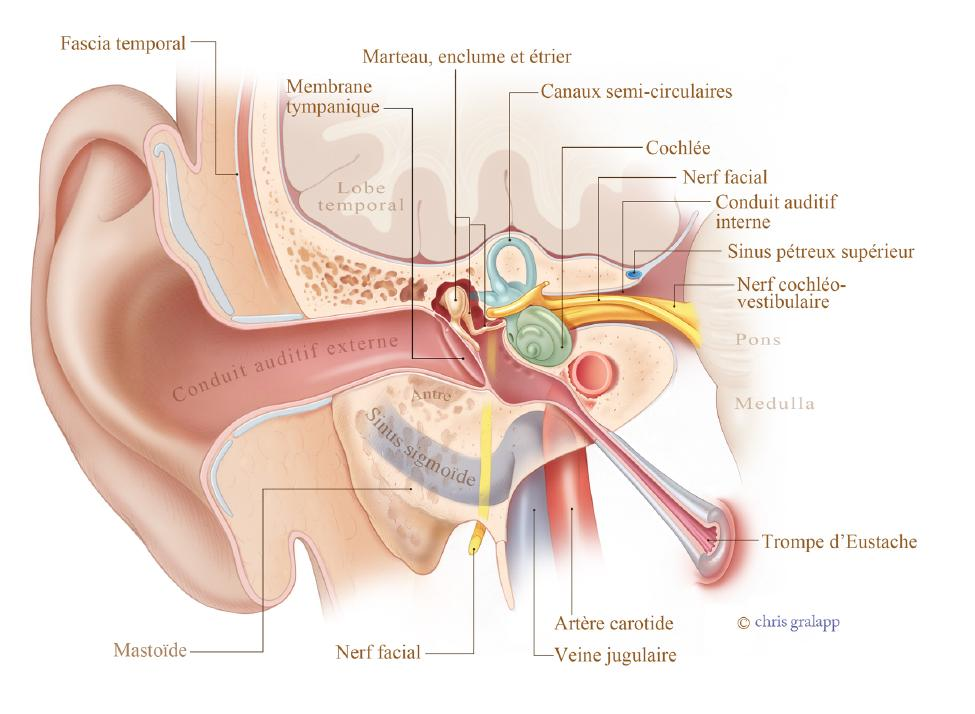
\includegraphics[width=1\linewidth]{images/20160624Berufsfeldgruppen.jpg}
	\caption[Anatomie oreille]{Anatomie de l'oreille}
	\label{fig:-20160624berufsfeldgruppen}
\end{figure}

L'oreille \autocite[ch. 8 pp. 319--321]{marieb:biologie} 
se situe à l'intérieur de l'un des os du crâne, le temporal, et plus précisément la pyramide pétreuse ou rocher. Elle se compose de trois parties : externe, moyenne, interne.

\subsubsection{L'oreille externe}

L'oreille externe\autocite[ch. 8, pp. 319--321.]{marieb:biologie}
est formée du pavillon et du méat acoustique externe
	(canal auditif). Les ondes sonores entrent dans le méat et percutent
	une membrane de \SI{60}{\milli\metre\squared}, appelée tympan, et la font vibrer. 
	Cette membrane
	sépare l'oreille externe de l'oreille moyenne. 


        Selon \textbf{Tomatis} 
	% au chapitre 3.3/ 4, 
	elle joue un rôle de filtre des graves et d'amplificateur des aigus.




\subsubsection{L'oreille moyenne}

L'oreille moyenne se trouve dans l'os temporal constituée de petites
cavités dont une, centrale, qui est la caisse du tympan. Sa limite
médiale est une paroi osseuse percée de deux orifices, la fenêtre
du vestibule et la fenêtre de la cochlée. La trompe auditive ou d'Eustache
est un conduit oblique qui relie l'oreille moyenne à la gorge et sert
à équilibrer la pression de l'air entre l'oreille moyenne et l'extérieur.
Les trois osselets de l'ouïe sont : le marteau, l'enclume et l'étrier
(les plus petits os du corps). Ils transmettent les vibrations du
tympan aux liquides de l'oreille interne.
Le marteau et l'étrier sont commandés chacun par un muscle.


Selon \textbf{Tomatis}, son rôle est double : protéger l'oreille interne des sons
trop forts et celui de cibler les sons à écouter.

\subsubsection{L'oreille interne et le labyrinthe osseux}

\begin{figure}
	\centering
	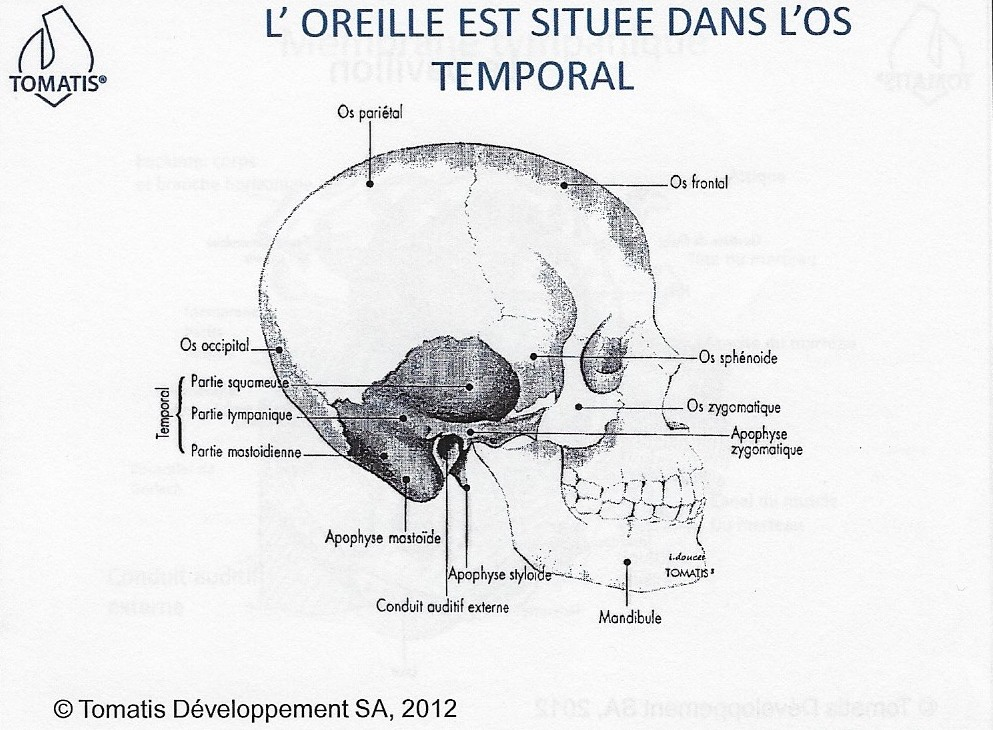
\includegraphics[width=0.7\linewidth]{images/Loreilleostemporal_crane.jpg}
	\caption[L'os temporal]{L'os temporal}
	\label{fig:loreilleostemporal18}
\end{figure}

L'oreille interne est l'organe de l'audition. Il
est constitué d'une coque osseuse d'une très grande densité (la plus
importante du corps), contenant un corps membraneux qui en épouse
la forme. 
L'oreille interne est une enfilade de cavités osseuses portant 
le nom de \emph{labyrinthe osseux}. Il comprend trois subdivisions : 
\begin{enumerate}
	\item la cochlée;
	\item le vestibule du labyrinthe;
	\item  les canaux semi-circulaires.
\end{enumerate}

Le labyrinthe
osseux est rempli de périlymphe, un liquide. Et dans ce périlymphe
flotte le labyrinthe membraneux qui contient lui-même un liquide
plus épais appelé endolymphe. Ils jouent leur rôle dans l'équilibre
statique et dynamique. Le vestibule et les canaux semi-circulaires
sont les organes de l'équilibration; la cochlée ou
limaçon est l'organe de l'audition. 

\subsubsection{Le canal auditif}
\pdfmargincomment[color=yellow]{répétition avec oreille externe}
Les ondes sonores entrent dans le méat et percutent
une membrane de \SI{60}{\milli\metre\squared} appelée \emph{tympan}, et la font vibrer. Cette membrane
sépare l'oreille externe de l'oreille moyenne.


Selon \textbf{Tomatis}, elle
joue un rôle de filtre des graves et d'amplificateur des aigus.



\subsection{La physiologie de l'audition}

Le  son crée un chemin dans 
l'oreille\autocite[chap. 8, pp. 322--324]{marieb:biologie} jusqu'au cerveau.

Chaque son parvenant à l'oreille entre dans le pavillon et se propage
dans le conduit auditif. Les vibrations de l'onde sonore mettent en
mouvement le tympan lié aux trois petits os (marteau, enclume, étrier).
Les osselets ont le rôle de transformer et d'amplifier les vibrations
aériennes et de les transmettre à l'oreille interne via la fenêtre
ovale.

Le rapport de levier effectif entre le marteau et l'enclume
(de l'ordre de 20), d'une part, et le
rapport de surfaces entre le tympan et la platine de l'étrier
(\SI{30}{\milli\metre\squared}) d\textquoteright autre part font du système tympano-ossiculaire
un véritable amplificateur permettant à l\textquoteright énergie sonore
d\textquoteright être transmise presque intégralement à l\textquoteright oreille
interne.

A partir de 80 dB, un réflexe protecteur (stapédien) est mis en place
afin de réduire la transmission des pressions vers l\textquoteright oreille
interne, par l\textquoteright intermédiaire des osselets et des muscles
qui rattachent le marteau et l\textquoteright étrier aux parois de
la caisse du tympan. Il s'agit ainsi d' un procédé mécanique qui amplifient
les vibrations atteignant la cochlée. 
\begin{quotation}
	La cochlée à son tour ``va transformer ces vibrations en impulsions
	nerveuses véhiculées par le nerf auditif.'' (\dots) Les cellules ciliées
	tapies dans la membrane cochléaire ``transforment ces vibrations
	en messages électriques, circulant dans le nerf auditif. (\dots) Et
	ces informations vont ``se diriger vers le cortex cérébral, via plusieurs
	relais. (\dots) ``Comme certaines fibres issues de chaque oreille croisent
	la ligne médiane, chaque aire auditive reçoit des signaux des deux
	oreilles.'' De plus, ``tout au long du trajet, le message subit
	des transformations dues aux caractéristiques de l'activité des neurones.''
	Retenons que `` les cellules ciliées proches de l'étrier sont activées
	par les sons aigus, et celles situées au sommet de la cochlée le sont
	par les sons de basse fréquence''. (\dots)``Une scène auditive est
	mêlée d'un ensemble d'ondes acoustiques et son analyse se ferait non
	seulement tout au long du système auditif avec des indices comme la
	fréquence et l'intensité mais aussi au-delà, pour utiliser les informations
	liées aux autres sens ou au contexte.'' \autocite[chap.1, pp.~15--16]{bigand:cerveau}
%	\footnote{\textbf{Le cerveau mélomane} Le cerveau mélomane,2011}, chap.1, pp.~15--16.}
\end{quotation}


        \begin{figure}
	\centering
	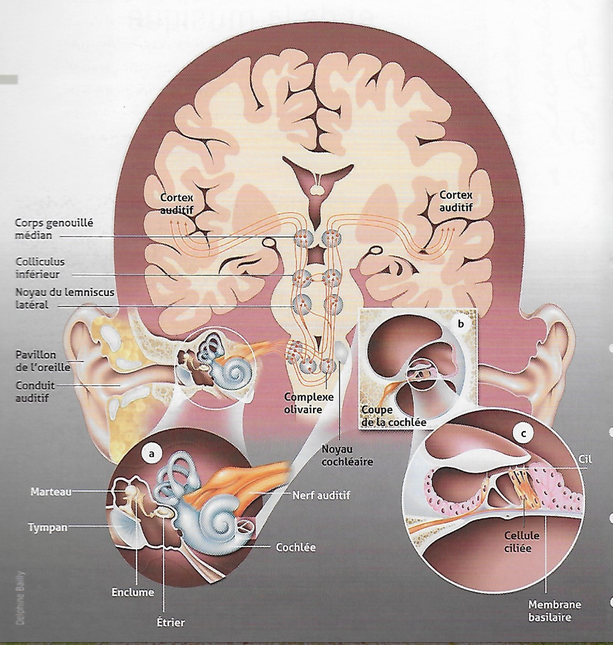
\includegraphics[width=1\linewidth]{images/schemacerveauoreillebigand.png}
	\caption[Schéma du déroulement]{La perception des sons et de
          la musique, E.Bigand, ``Le cerveau mélomane''Ed.Belin}
       
	\label{cerveauoreillebigand1}
\end{figure}




\chapter{Acoustique}

\section{Courbe de Wegel}
\label{acoustique}

<<Effectivement la courbe de Wegel est la courbe de réponse obtenue
lorsque sont posées en abscisses les fréquences, et en ordonnées ascendantes
les intensités. Un premier seuil s'obtient, en partie basse, suivant
un minimum qui commence dans les fréquences graves à environ 
\SIrange{40}{50}{\dB}, avoisine ensuite la courbe des abscisses entre 2000 et \SI{3000}{\Hz}
et redevient ascendante à \SI{40}{\decibel} / \SI{50}{\decibel} dans les aigus entre \SI{8000}{\Hz} et
\SI{10000}{\Hz}. Cette courbe se complète et prend l'allure de citron selon
l'expression qu'on lui confère lorsqu'on envoie des
sons d'intensité croissante et qu'on obtient alors une courbe des
seuils maxima qui se déterminent là où l'oreille commence à souffrir,
d'où le nom de ``seuil de la douleur". Ces seuils
commencent dans les graves, également de \SIrange{50}{60}{\decibel}, rejoignant la première
courbe, puis ils atteignent \SIrange{120}{130}{\decibel} entre \SI{2000}{\Hz} et \SI{3000}{\Hz} pour
chuter ensuite dans les aigus en rejoignant également la première
courbe. La ligne médiane qui se situe aux environs de \SIrange{50}{60}{\dB}, qui
est linéaire représente une zone dite ``Zone de Munsen''.
Elle répond à la dynamique de l'oreille, c'est-à-dire
à sa zone ``optimale" de fonctionnement sans
distorsion. Dans toutes les autres zones, l'oreille
agit comme un filtre dont les pentes sont variables en fonction de
l'intensité, avec un lieu de rotation situé de \SIrange{1000}{2000}{\Hz}. Pour pallier ces distorsions toujours difficiles à intégrer
dans la lecture des schémas, les Américains ont standardisé les audiogrammes
du type de ceux que nous utilisons tous en inversant l'image
de Wegel et en redressant les \emph{minima} pour obtenir une ligne droite.
Ces normes gardent néanmoins une zone préférentielle de \SIrange{1000}{2000}{\Hz} malgré les compensations de \SIrange{30}{40}{\dB} accordées sur la courbe,
dans les graves et les aigus.>>
\autocite[Bernard Auriol, conversation, conférence]{auriol_stress}.

% OGA: stp la source bibliographique ou conférence

\section{Impédance}
\label{impedance}

Définition de l'impédance : L'impédance acoustique
caractérise la résistance qu'un milieu oppose à sa mise en mouvement
lorsqu'il est traversé par une onde acoustique. Elle est définie comme
le rapport de la pression acoustique sur la vitesse de déplacement
locale dans un milieu, et est généralement notée $Z$. Elle dépend de
la température. L'impédance caractéristique d'un milieu (solide, liquide
ou gazeux) est définie comme le rapport de la pression acoustique
sur la vitesse de déplacement en milieu ouvert (c'est-à-dire
en l'absence d'ondes réfléchies). L'impédance caractéristique est
une propriété du matériau considéré égale, dans le cas d'un espace
illimité, au produit de la masse volumique du matériau $\rho$
par la vitesse du son $c$ dans ce même matériau : $Z = \rho_{m} c$.

Unités : $\rho_{m}$ étant exprimé en \si{kg/m\cubed},
$c$ en \si{m/s}, $Z$ est
exprimé en \si{\pascal . s/m}.
\chapter{Feuille informative de l'étude faite à la Privatklinik von Meiringen}
Voici la version originale en allemand proposée aux patients:
\begin{german}

Information für Mitwirkende an der klinischen Studie
\foreignquote{german}{Evaluierung des aktiven Hörvermögens}


Sehr geehrte Damen und Herren,

Herzlichen Dank für Ihr Interesse an dieser Studie !

Wozu dient diese Studie und weshalb werden Sie um eine Teilnahme gebeten ?

Während Ihrem Klinikaufenthalt  in der Privatklinik von Meiringen werden Sie im Kontext 
unseres multidisziplinären Teams verschiedene Therapien besuchen, unter anderem auch die Musiktherapie. Bei der vorliegenden Studie möchten wir untersuchen, wie sich die Musiktherapie auf Ihr Zuhörvermögen auswirkt.
Musiktherapie ist eine gut erforschte Intervention im Bereich des Depressions und Burnouts, da Sie ein relativ neues Berufsfeld ist, gibt es noch viel Forschungspotential.
Das Hörtest konnte sich als ein Instrument erweisen, um die Veränderung des Gehörs des Patienten bei einer Musiktherapiebehandlung zu beweisen. Die Verbindung dieses Ansatzes mit der Musiktherapie ist noch nicht erforscht und daher soll dieser Ansatz wissenschaftlich näher untersucht werden.
Wenn Sie keine Musiktherapie besuchen aber Interesse für diese Studie haben, sind Sie herzlich eingeladen, dieses Test zu tun. Im Rahmen under MAS brauchen wir unbedingt eine Kontrollgruppe.

Wie sieht eine Teilnahme an der Studie aus ?

Die Untersuchung erfolgt sehr einfach in mehreren Schritten.
Zu Verfügung steht ein Apparat, mit dem sich spezifische Hörtests durchführen lassen.
Allgemein Verlauf des Tests :  
Sie hören einen sehr leisen Ton mit Zuhörern zu und werden ihn entweder mit der rechten  oder linken Hand  signalisieren. Das dauert ungefähr 30 Minuten.
Es wird zwei Tests geben : ein vor der Therapie und ein nach der Therapie.
Wir bitten Sie auch, eine kleine Fragebogen zu erfüllen.


Falls Sie Fragen haben, dürfen Sie sich gerne via E-Mail melden : valerie.gaillard\@gmx.ch

Wir bedanken uns herzlich für Ihre Zeit und die Teilnahme an dieser Studie.

\end{german}
Valérie Gaillard


\textgerman{ZhdK : Upgrade MAS Klinische Musiktherapie 15-17}

\section{Feuille informative en français de l'étude faite à la Privatklinik von Meiringen}

Information pour les participants à l'étude clinique
\foreignquote{french}{Evaluation de la capacité de l'écoute active}


Mesdames et Messieurs,

Tout d'abord un très grand merci pour votre intérêt à cette étude!

Dans quels buts et pour quelles raisons êtes-vous priés de participer à
cette étude?

Pendant votre séjour à la clinique de Meiringen, vous allez prendre
part dans le contexte multidisciplinaire à différentes thérapies, dont
la musicothérapie. Avec l'étude présente, nous aimerions étudier comment
la musicothérapie agit sur vos capacités d'écoute.
La musicothérapie fait partie des interventions indiquées et explorées dans le domaine
de la dépression et du burnout; comme c'est un champ
professionnel
relativement nouveau, (il existe un grand potentiel de recherche.) nous avons encore de grandes possibilités d'investigation.
Le test d'écoute pourrait être un instrument prouvant et démontrant le changement
d'écoute du patient lors d'un traitement en musicothérapie.
Le lien de cette approche avec la musicothérapie n'a pas été encore
investigué et c'est la raison pour laquelle elle mérite d'être
recherchée beaucoup plus en profondeur.

Si vous ne suivez aucune musicothérapie mais que vous êtes intéressés
par cette étude, vous êtes invités cordialement à faire ce test. Dans
le cadre de ce travail, il est nécessaire d'avoir un groupe de contrôle.

Comment se présente une participation à cette étude ?

L'étude se déroule très simplement en plusieurs étapes:
À disposition se tient un appareil, avec lequel se fait un test spécifique d'écoute.

Déroulement général du test :
Vous entendrez  avec des écouteurs un son de très faible intensité, que
vous devrez signaler avec la main droite ou gauche, du côté
perçu.
Le tout dure environ 30mn.
Il y aura 2 tests: un avant la thérapie et l'autre après, et à chaque
fois, il sera nécessaire de remplir un petit questionnaire.
Nous vous prions également de signer votre consentement avant le début
de l'étude.


Au cas où vous avez des questions, écrivez-les par E-Mail à cette adresse : valerie.gaillard\@gmx.ch

Nous vous remercions d'ores et déjà beaucoup pour votre participation
à cette étude.

Valérie Gaillard


\begin{french}
	Le matériel utilisé : une table, deux chaises, l'appareil
	test Hearing et les deux écouteurs: l'un aérien et l'autre osseux, un crayon, deux
	feutres (rouge et bleu), une feuille avec la grille de fréquences à
	remplir.
\end{french}

\chapter{WHOQO--Bref: World Health
   Organisation Quality of Life Assessement}

Le WHOQO--Bref (World Health
   Organisation Quality of Life Assessement) est ici reproduite en
   français et en
   version allemande, telle qu'elle a été présentée aux patients.

\includepdfmerge{French_WHOQOL-BREF.pdf, -, 
 WHOQOLALLEMANDBREFupdated.pdf, -}

Le WHOQO--Bref (World Health
   Organisation Quality of Life Assessement) est ici reproduite en
   français et en
   version allemande, telle qu'elle a été présentée aux patients.

\chapter{Déclaration de consentement}

\begin{figure}
	\centering
	\includegraphics[width=1\linewidth]{images/einverstandniserkl.jpg}
	\caption{Déclaration de consentement écrite concernant la
          participation à l'investigation}
	\label{fig:déclaration de consentement}
\end{figure}
%\includepdfmerge{French_WHOQOL-BREF.pdf, -}
%\includepdfmerge{WHOQOLALLEMANDBREFupdated.pdf, -}

%\section{Questionnaire 1}
%
%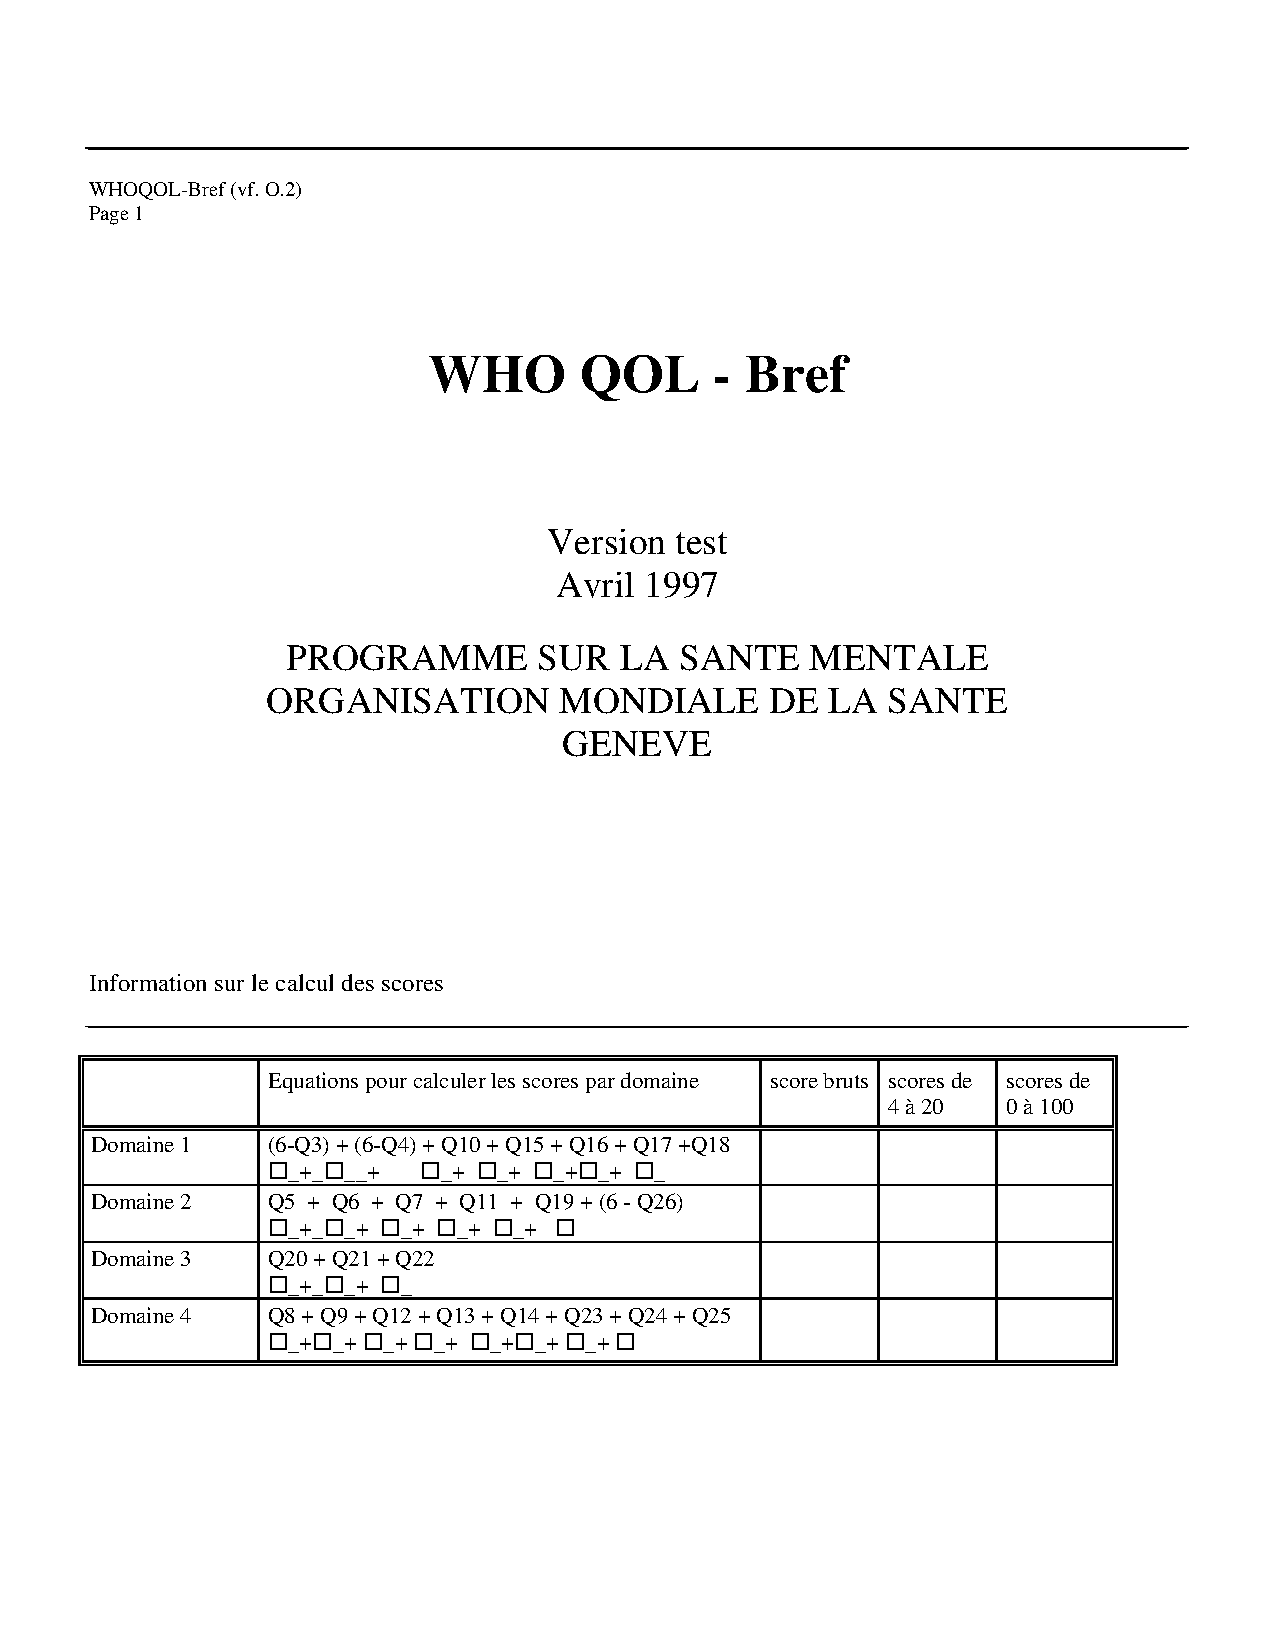
\includepdf[pages=-]{French_WHOQOL-BREF.pdf}
%
%\section{Questionnaire 2}
%
%
\includepdf[pages=-]{WHOQOLALLEMANDBREFupdated.pdf}

\chapter{Travail passif et actif de la méthode Tomatis}

\begin{description}
\item [{1\iere session}] de 25 à 30h d'écoute : le patient écoute
deux heures de musique par jour pendant 13 à 15 jours consécutifs;
un deuxième test à la fin de ce travail; ensuite, une pause pendant
4 à 6 semaines.
\item [{2\ieme session}] de 25 à 30h d'écoute : 3ieme Test, à nouveau
deux heures d'écoute pendant 13 jours à 15 jours; puis 4\ieme test,
suivi d'une pause d'une durée de 4 à 8 semaines.
\item [{3\ieme session}] : la même façon de procéder que les deux
autres. 
\end{description}

Le choix et le traitement des musiques peuvent être très différents
selon le patient et sa pathologie.

%\selectlanguage{french}
\nocite{*} % imprime toute la bibliographie et pas seulement
% les livres cités
\phantomsection 
\addcontentsline{toc}{chapter}{Bibliographie} 
\label{bibliographie}
\printbibliography
\end{document}
